% Options for packages loaded elsewhere
\PassOptionsToPackage{unicode}{hyperref}
\PassOptionsToPackage{hyphens}{url}
\PassOptionsToPackage{dvipsnames,svgnames,x11names}{xcolor}
%
\documentclass[
  ignorenonframetext,
]{beamer}
\usepackage{pgfpages}
\setbeamertemplate{caption}[numbered]
\setbeamertemplate{caption label separator}{: }
\setbeamercolor{caption name}{fg=normal text.fg}
\beamertemplatenavigationsymbolsempty
% Prevent slide breaks in the middle of a paragraph
\widowpenalties 1 10000
\raggedbottom
\setbeamertemplate{part page}{
  \centering
  \begin{beamercolorbox}[sep=16pt,center]{part title}
    \usebeamerfont{part title}\insertpart\par
  \end{beamercolorbox}
}
\setbeamertemplate{section page}{
  \centering
  \begin{beamercolorbox}[sep=12pt,center]{part title}
    \usebeamerfont{section title}\insertsection\par
  \end{beamercolorbox}
}
\setbeamertemplate{subsection page}{
  \centering
  \begin{beamercolorbox}[sep=8pt,center]{part title}
    \usebeamerfont{subsection title}\insertsubsection\par
  \end{beamercolorbox}
}
\AtBeginPart{
  \frame{\partpage}
}
\AtBeginSection{
  \ifbibliography
  \else
    \frame{\sectionpage}
  \fi
}
\AtBeginSubsection{
  \frame{\subsectionpage}
}
\usepackage{amsmath,amssymb}
\usepackage{lmodern}
\usepackage{iftex}
\ifPDFTeX
  \usepackage[T1]{fontenc}
  \usepackage[utf8]{inputenc}
  \usepackage{textcomp} % provide euro and other symbols
\else % if luatex or xetex
  \usepackage{unicode-math}
  \defaultfontfeatures{Scale=MatchLowercase}
  \defaultfontfeatures[\rmfamily]{Ligatures=TeX,Scale=1}
\fi
% Use upquote if available, for straight quotes in verbatim environments
\IfFileExists{upquote.sty}{\usepackage{upquote}}{}
\IfFileExists{microtype.sty}{% use microtype if available
  \usepackage[]{microtype}
  \UseMicrotypeSet[protrusion]{basicmath} % disable protrusion for tt fonts
}{}
\makeatletter
\@ifundefined{KOMAClassName}{% if non-KOMA class
  \IfFileExists{parskip.sty}{%
    \usepackage{parskip}
  }{% else
    \setlength{\parindent}{0pt}
    \setlength{\parskip}{6pt plus 2pt minus 1pt}}
}{% if KOMA class
  \KOMAoptions{parskip=half}}
\makeatother
\usepackage{xcolor}
\newif\ifbibliography
\usepackage{color}
\usepackage{fancyvrb}
\newcommand{\VerbBar}{|}
\newcommand{\VERB}{\Verb[commandchars=\\\{\}]}
\DefineVerbatimEnvironment{Highlighting}{Verbatim}{commandchars=\\\{\}}
% Add ',fontsize=\small' for more characters per line
\usepackage{framed}
\definecolor{shadecolor}{RGB}{248,248,248}
\newenvironment{Shaded}{\begin{snugshade}}{\end{snugshade}}
\newcommand{\AlertTok}[1]{\textcolor[rgb]{0.94,0.16,0.16}{#1}}
\newcommand{\AnnotationTok}[1]{\textcolor[rgb]{0.56,0.35,0.01}{\textbf{\textit{#1}}}}
\newcommand{\AttributeTok}[1]{\textcolor[rgb]{0.77,0.63,0.00}{#1}}
\newcommand{\BaseNTok}[1]{\textcolor[rgb]{0.00,0.00,0.81}{#1}}
\newcommand{\BuiltInTok}[1]{#1}
\newcommand{\CharTok}[1]{\textcolor[rgb]{0.31,0.60,0.02}{#1}}
\newcommand{\CommentTok}[1]{\textcolor[rgb]{0.56,0.35,0.01}{\textit{#1}}}
\newcommand{\CommentVarTok}[1]{\textcolor[rgb]{0.56,0.35,0.01}{\textbf{\textit{#1}}}}
\newcommand{\ConstantTok}[1]{\textcolor[rgb]{0.00,0.00,0.00}{#1}}
\newcommand{\ControlFlowTok}[1]{\textcolor[rgb]{0.13,0.29,0.53}{\textbf{#1}}}
\newcommand{\DataTypeTok}[1]{\textcolor[rgb]{0.13,0.29,0.53}{#1}}
\newcommand{\DecValTok}[1]{\textcolor[rgb]{0.00,0.00,0.81}{#1}}
\newcommand{\DocumentationTok}[1]{\textcolor[rgb]{0.56,0.35,0.01}{\textbf{\textit{#1}}}}
\newcommand{\ErrorTok}[1]{\textcolor[rgb]{0.64,0.00,0.00}{\textbf{#1}}}
\newcommand{\ExtensionTok}[1]{#1}
\newcommand{\FloatTok}[1]{\textcolor[rgb]{0.00,0.00,0.81}{#1}}
\newcommand{\FunctionTok}[1]{\textcolor[rgb]{0.00,0.00,0.00}{#1}}
\newcommand{\ImportTok}[1]{#1}
\newcommand{\InformationTok}[1]{\textcolor[rgb]{0.56,0.35,0.01}{\textbf{\textit{#1}}}}
\newcommand{\KeywordTok}[1]{\textcolor[rgb]{0.13,0.29,0.53}{\textbf{#1}}}
\newcommand{\NormalTok}[1]{#1}
\newcommand{\OperatorTok}[1]{\textcolor[rgb]{0.81,0.36,0.00}{\textbf{#1}}}
\newcommand{\OtherTok}[1]{\textcolor[rgb]{0.56,0.35,0.01}{#1}}
\newcommand{\PreprocessorTok}[1]{\textcolor[rgb]{0.56,0.35,0.01}{\textit{#1}}}
\newcommand{\RegionMarkerTok}[1]{#1}
\newcommand{\SpecialCharTok}[1]{\textcolor[rgb]{0.00,0.00,0.00}{#1}}
\newcommand{\SpecialStringTok}[1]{\textcolor[rgb]{0.31,0.60,0.02}{#1}}
\newcommand{\StringTok}[1]{\textcolor[rgb]{0.31,0.60,0.02}{#1}}
\newcommand{\VariableTok}[1]{\textcolor[rgb]{0.00,0.00,0.00}{#1}}
\newcommand{\VerbatimStringTok}[1]{\textcolor[rgb]{0.31,0.60,0.02}{#1}}
\newcommand{\WarningTok}[1]{\textcolor[rgb]{0.56,0.35,0.01}{\textbf{\textit{#1}}}}
\usepackage{graphicx}
\makeatletter
\def\maxwidth{\ifdim\Gin@nat@width>\linewidth\linewidth\else\Gin@nat@width\fi}
\def\maxheight{\ifdim\Gin@nat@height>\textheight\textheight\else\Gin@nat@height\fi}
\makeatother
% Scale images if necessary, so that they will not overflow the page
% margins by default, and it is still possible to overwrite the defaults
% using explicit options in \includegraphics[width, height, ...]{}
\setkeys{Gin}{width=\maxwidth,height=\maxheight,keepaspectratio}
% Set default figure placement to htbp
\makeatletter
\def\fps@figure{htbp}
\makeatother
\setlength{\emergencystretch}{3em} % prevent overfull lines
\providecommand{\tightlist}{%
  \setlength{\itemsep}{0pt}\setlength{\parskip}{0pt}}
\setcounter{secnumdepth}{-\maxdimen} % remove section numbering
\usepackage{graphicx}
\usepackage{bm}
\definecolor{foreground}{RGB}{255,255,255}
\definecolor{background}{RGB}{34,28,54}
\definecolor{title}{RGB}{105,165,255}
\definecolor{gray}{RGB}{175,175,175}
\definecolor{lightgray}{RGB}{225,225,225}
\definecolor{subtitle}{RGB}{232,234,255}
\definecolor{hilight}{RGB}{112,224,255}
\definecolor{vhilight}{RGB}{255,111,207}
\setbeamertemplate{footline}[page number]
\usepackage{amsthm}
\usepackage{amsmath}
\usepackage{amsfonts}
\usepackage{amscd}
\usepackage{amssymb}
\usepackage{natbib}
\usepackage{url}
\usepackage{tikz}
\ifLuaTeX
  \usepackage{selnolig}  % disable illegal ligatures
\fi
\IfFileExists{bookmark.sty}{\usepackage{bookmark}}{\usepackage{hyperref}}
\IfFileExists{xurl.sty}{\usepackage{xurl}}{} % add URL line breaks if available
\urlstyle{same} % disable monospaced font for URLs
\hypersetup{
  pdftitle={STAT 528 - Advanced Regression Analysis II},
  pdfauthor={Aster models},
  colorlinks=true,
  linkcolor={Maroon},
  filecolor={Maroon},
  citecolor={Blue},
  urlcolor={blue},
  pdfcreator={LaTeX via pandoc}}

\title{STAT 528 - Advanced Regression Analysis II}
\author{Aster models}
\date{}
\institute{Daniel J. Eck\\
Department of Statistics\\
University of Illinois}

\begin{document}
\frame{\titlepage}

\begin{frame}
\newcommand{\R}{\mathbb{R}}
\end{frame}

\begin{frame}{Learning Objectives Today}
\protect\hypertarget{learning-objectives-today}{}
\begin{itemize}
\tightlist
\item
  aster model example
\item
  aster analysis
\end{itemize}
\end{frame}

\begin{frame}{}
\protect\hypertarget{section}{}
The variables under consideration:

\begin{itemize}
\tightlist
\item
  \texttt{nsloc} north-south location of each individual in the
  experimental plot
\item
  \texttt{ewloc} east-west location of each individual in the
  experimental plot
\item
  \texttt{pop} the ancestral population of each individual
\end{itemize}

\vspace{12pt}

Each individual was grown from seed taken from a surviving population in
a prairie remnant in western Minnesota near the Echinacea Project field
site.

Darwinian fitness (our best surrogate of Darwinian fitness) is total
flower head count over the years of data collection.

We are interested in estimated expected Darwinian fitness for the
different ancestral populations.
\end{frame}

\begin{frame}{The aster graph for \emph{Echinacea angustifolia}
(\href{http://echinaceaproject.org/}{aster plants})}
\protect\hypertarget{the-aster-graph-for-aster-plants}{}
\begin{figure}
\begin{tikzpicture}
\put(-100,50){\makebox(0,0){$1$}}
\put(-50,50){\makebox(0,0){$M_1$}}
\put(0,50){\makebox(0,0){$M_2$}}
\put(50,50){\makebox(0,0){$M_3$}}
\put(-87.5,50){\vector(1,0){25}}
\put(-37.5,50){\vector(1,0){25}}
\put(12.5,50){\vector(1,0){25}}
\put(-50,0){\makebox(0,0){$F_1$}}
\put(0,0){\makebox(0,0){$F_2$}}
\put(50,0){\makebox(0,0){$F_3$}}
\put(-50,37.5){\vector(0,-1){25}}
\put(0,37.5){\vector(0,-1){25}}
\put(50,37.5){\vector(0,-1){25}}
\put(-50,-50){\makebox(0,0){$H_1$}}
\put(0,-50){\makebox(0,0){$H_2$}}
\put(50,-50){\makebox(0,0){$H_3$}}
\put(-50,-12.5){\vector(0,-1){25}}
\put(0,-12.5){\vector(0,-1){25}}
\put(50,-12.5){\vector(0,-1){25}}
\end{tikzpicture}
\label{fig:astergraph}
\end{figure}
\end{frame}

\begin{frame}[fragile]{}
\protect\hypertarget{section-1}{}
We load in necessary packages:

\vspace{12pt}

\begin{Shaded}
\begin{Highlighting}[]
\FunctionTok{library}\NormalTok{(tidyverse)}
\FunctionTok{library}\NormalTok{(ggplot2)}
\FunctionTok{library}\NormalTok{(aster)}
\FunctionTok{library}\NormalTok{(aster2)}
\end{Highlighting}
\end{Shaded}
\end{frame}

\begin{frame}[fragile]{Initial data processing}
\protect\hypertarget{initial-data-processing}{}
Here is a brief look at the data:

\vspace{12pt}
\tiny

\begin{Shaded}
\begin{Highlighting}[]
\FunctionTok{data}\NormalTok{(}\StringTok{"echinacea"}\NormalTok{)}
\FunctionTok{names}\NormalTok{(echinacea)}
\end{Highlighting}
\end{Shaded}

\begin{verbatim}
##  [1] "redata"        "repred"        "regroup"       "recode"       
##  [5] "families"      "redelta"       "initial"       "response.name"
##  [9] "pred"          "group"         "code"
\end{verbatim}

\begin{Shaded}
\begin{Highlighting}[]
\FunctionTok{head}\NormalTok{(echinacea}\SpecialCharTok{$}\NormalTok{redata)}
\end{Highlighting}
\end{Shaded}

\begin{verbatim}
##           pop ewloc nsloc varb resp id
## 1.ld02   NWLF    -8   -11 ld02    0  1
## 2.ld02 Eriley    -8   -10 ld02    1  2
## 3.ld02   NWLF    -8    -9 ld02    0  3
## 4.ld02    SPP    -8    -8 ld02    0  4
## 5.ld02    SPP    -8    -7 ld02    0  5
## 6.ld02 Eriley    -8    -6 ld02    1  6
\end{verbatim}
\end{frame}

\begin{frame}[fragile]{}
\protect\hypertarget{section-2}{}
\tiny

\begin{Shaded}
\begin{Highlighting}[]
\NormalTok{echinacea}\SpecialCharTok{$}\NormalTok{redata }\SpecialCharTok{\%\textgreater{}\%} \FunctionTok{filter}\NormalTok{(id }\SpecialCharTok{==} \DecValTok{1}\NormalTok{)}
\end{Highlighting}
\end{Shaded}

\begin{verbatim}
##           pop ewloc nsloc   varb resp id
## 1.ld02   NWLF    -8   -11   ld02    0  1
## 1.ld03   NWLF    -8   -11   ld03    0  1
## 1.ld04   NWLF    -8   -11   ld04    0  1
## 1.fl02   NWLF    -8   -11   fl02    0  1
## 1.fl03   NWLF    -8   -11   fl03    0  1
## 1.fl04   NWLF    -8   -11   fl04    0  1
## 1.hdct02 NWLF    -8   -11 hdct02    0  1
## 1.hdct03 NWLF    -8   -11 hdct03    0  1
## 1.hdct04 NWLF    -8   -11 hdct04    0  1
\end{verbatim}

\begin{Shaded}
\begin{Highlighting}[]
\NormalTok{echinacea}\SpecialCharTok{$}\NormalTok{redata }\SpecialCharTok{\%\textgreater{}\%} \FunctionTok{filter}\NormalTok{(id }\SpecialCharTok{==} \DecValTok{6}\NormalTok{)}
\end{Highlighting}
\end{Shaded}

\begin{verbatim}
##             pop ewloc nsloc   varb resp id
## 6.ld02   Eriley    -8    -6   ld02    1  6
## 6.ld03   Eriley    -8    -6   ld03    1  6
## 6.ld04   Eriley    -8    -6   ld04    1  6
## 6.fl02   Eriley    -8    -6   fl02    0  6
## 6.fl03   Eriley    -8    -6   fl03    0  6
## 6.fl04   Eriley    -8    -6   fl04    1  6
## 6.hdct02 Eriley    -8    -6 hdct02    0  6
## 6.hdct03 Eriley    -8    -6 hdct03    0  6
## 6.hdct04 Eriley    -8    -6 hdct04    1  6
\end{verbatim}
\end{frame}

\begin{frame}[fragile]{}
\protect\hypertarget{section-3}{}
We can see the proportion of individuals that survive each year.

\vspace{12pt}
\tiny

\begin{Shaded}
\begin{Highlighting}[]
\DocumentationTok{\#\# M1}
\NormalTok{echinacea}\SpecialCharTok{$}\NormalTok{redata }\SpecialCharTok{\%\textgreater{}\%} \FunctionTok{filter}\NormalTok{(varb }\SpecialCharTok{==} \StringTok{"ld02"}\NormalTok{) }\SpecialCharTok{\%\textgreater{}\%} \FunctionTok{pull}\NormalTok{(resp) }\SpecialCharTok{\%\textgreater{}\%} \FunctionTok{table}\NormalTok{()}
\end{Highlighting}
\end{Shaded}

\begin{verbatim}
## .
##   0   1 
## 158 412
\end{verbatim}

\begin{Shaded}
\begin{Highlighting}[]
\DocumentationTok{\#\# M2}
\NormalTok{echinacea}\SpecialCharTok{$}\NormalTok{redata }\SpecialCharTok{\%\textgreater{}\%} \FunctionTok{filter}\NormalTok{(id }\SpecialCharTok{\%in\%}\NormalTok{ (echinacea}\SpecialCharTok{$}\NormalTok{redata }\SpecialCharTok{\%\textgreater{}\%} 
                                       \FunctionTok{filter}\NormalTok{(varb }\SpecialCharTok{==} \StringTok{"ld02"} \SpecialCharTok{\&}\NormalTok{ resp }\SpecialCharTok{==} \DecValTok{1}\NormalTok{) }\SpecialCharTok{\%\textgreater{}\%} 
                                       \FunctionTok{pull}\NormalTok{(id)) }\SpecialCharTok{\&}\NormalTok{ varb }\SpecialCharTok{==} \StringTok{"ld03"}\NormalTok{) }\SpecialCharTok{\%\textgreater{}\%} 
  \FunctionTok{pull}\NormalTok{(resp) }\SpecialCharTok{\%\textgreater{}\%} \FunctionTok{table}\NormalTok{()}
\end{Highlighting}
\end{Shaded}

\begin{verbatim}
## .
##   0   1 
##  20 392
\end{verbatim}

\begin{Shaded}
\begin{Highlighting}[]
\DocumentationTok{\#\# M3}
\NormalTok{echinacea}\SpecialCharTok{$}\NormalTok{redata }\SpecialCharTok{\%\textgreater{}\%} \FunctionTok{filter}\NormalTok{(id }\SpecialCharTok{\%in\%}\NormalTok{ (echinacea}\SpecialCharTok{$}\NormalTok{redata }\SpecialCharTok{\%\textgreater{}\%} 
                                       \FunctionTok{filter}\NormalTok{(varb }\SpecialCharTok{==} \StringTok{"ld03"} \SpecialCharTok{\&}\NormalTok{ resp }\SpecialCharTok{==} \DecValTok{1}\NormalTok{) }\SpecialCharTok{\%\textgreater{}\%} 
                                       \FunctionTok{pull}\NormalTok{(id)) }\SpecialCharTok{\&}\NormalTok{ varb }\SpecialCharTok{==} \StringTok{"ld04"}\NormalTok{) }\SpecialCharTok{\%\textgreater{}\%} 
  \FunctionTok{pull}\NormalTok{(resp) }\SpecialCharTok{\%\textgreater{}\%} \FunctionTok{table}\NormalTok{()}
\end{Highlighting}
\end{Shaded}

\begin{verbatim}
## .
##   0   1 
##  14 378
\end{verbatim}
\end{frame}

\begin{frame}[fragile]{}
\protect\hypertarget{section-4}{}
We can see the proportion of individuals that flower each year.

\vspace{12pt}
\tiny

\begin{Shaded}
\begin{Highlighting}[]
\DocumentationTok{\#\# F1}
\NormalTok{echinacea}\SpecialCharTok{$}\NormalTok{redata }\SpecialCharTok{\%\textgreater{}\%} \FunctionTok{filter}\NormalTok{(id }\SpecialCharTok{\%in\%}\NormalTok{ (echinacea}\SpecialCharTok{$}\NormalTok{redata }\SpecialCharTok{\%\textgreater{}\%} 
                                       \FunctionTok{filter}\NormalTok{(varb }\SpecialCharTok{==} \StringTok{"ld02"} \SpecialCharTok{\&}\NormalTok{ resp }\SpecialCharTok{==} \DecValTok{1}\NormalTok{) }\SpecialCharTok{\%\textgreater{}\%} 
                                       \FunctionTok{pull}\NormalTok{(id)) }\SpecialCharTok{\&}\NormalTok{ varb }\SpecialCharTok{==} \StringTok{"fl02"}\NormalTok{) }\SpecialCharTok{\%\textgreater{}\%} 
  \FunctionTok{pull}\NormalTok{(resp) }\SpecialCharTok{\%\textgreater{}\%} \FunctionTok{table}\NormalTok{()}
\end{Highlighting}
\end{Shaded}

\begin{verbatim}
## .
##   0   1 
## 253 159
\end{verbatim}

\begin{Shaded}
\begin{Highlighting}[]
\DocumentationTok{\#\# F2}
\NormalTok{echinacea}\SpecialCharTok{$}\NormalTok{redata }\SpecialCharTok{\%\textgreater{}\%} \FunctionTok{filter}\NormalTok{(id }\SpecialCharTok{\%in\%}\NormalTok{ (echinacea}\SpecialCharTok{$}\NormalTok{redata }\SpecialCharTok{\%\textgreater{}\%} 
                                       \FunctionTok{filter}\NormalTok{(varb }\SpecialCharTok{==} \StringTok{"ld03"} \SpecialCharTok{\&}\NormalTok{ resp }\SpecialCharTok{==} \DecValTok{1}\NormalTok{) }\SpecialCharTok{\%\textgreater{}\%} 
                                       \FunctionTok{pull}\NormalTok{(id)) }\SpecialCharTok{\&}\NormalTok{ varb }\SpecialCharTok{==} \StringTok{"fl03"}\NormalTok{) }\SpecialCharTok{\%\textgreater{}\%} 
  \FunctionTok{pull}\NormalTok{(resp) }\SpecialCharTok{\%\textgreater{}\%} \FunctionTok{table}\NormalTok{()}
\end{Highlighting}
\end{Shaded}

\begin{verbatim}
## .
##   0   1 
## 266 126
\end{verbatim}

\begin{Shaded}
\begin{Highlighting}[]
\DocumentationTok{\#\# F3}
\NormalTok{echinacea}\SpecialCharTok{$}\NormalTok{redata }\SpecialCharTok{\%\textgreater{}\%} \FunctionTok{filter}\NormalTok{(id }\SpecialCharTok{\%in\%}\NormalTok{ (echinacea}\SpecialCharTok{$}\NormalTok{redata }\SpecialCharTok{\%\textgreater{}\%} 
                                       \FunctionTok{filter}\NormalTok{(varb }\SpecialCharTok{==} \StringTok{"ld04"} \SpecialCharTok{\&}\NormalTok{ resp }\SpecialCharTok{==} \DecValTok{1}\NormalTok{) }\SpecialCharTok{\%\textgreater{}\%} 
                                       \FunctionTok{pull}\NormalTok{(id)) }\SpecialCharTok{\&}\NormalTok{ varb }\SpecialCharTok{==} \StringTok{"fl04"}\NormalTok{) }\SpecialCharTok{\%\textgreater{}\%} 
  \FunctionTok{pull}\NormalTok{(resp) }\SpecialCharTok{\%\textgreater{}\%} \FunctionTok{table}\NormalTok{()}
\end{Highlighting}
\end{Shaded}

\begin{verbatim}
## .
##   0   1 
## 162 216
\end{verbatim}
\end{frame}

\begin{frame}[fragile]{}
\protect\hypertarget{section-5}{}
We can see the distribution of head counts each year.

\vspace{12pt}
\tiny

\begin{Shaded}
\begin{Highlighting}[]
\NormalTok{echinacea}\SpecialCharTok{$}\NormalTok{redata }\SpecialCharTok{\%\textgreater{}\%} \FunctionTok{filter}\NormalTok{(id }\SpecialCharTok{\%in\%}\NormalTok{ (echinacea}\SpecialCharTok{$}\NormalTok{redata }\SpecialCharTok{\%\textgreater{}\%} 
                                       \FunctionTok{filter}\NormalTok{(varb }\SpecialCharTok{==} \StringTok{"fl02"} \SpecialCharTok{\&}\NormalTok{ resp }\SpecialCharTok{==} \DecValTok{1}\NormalTok{) }\SpecialCharTok{\%\textgreater{}\%} 
                                       \FunctionTok{pull}\NormalTok{(id)) }\SpecialCharTok{\&}\NormalTok{ varb }\SpecialCharTok{==} \StringTok{"hdct02"}\NormalTok{) }\SpecialCharTok{\%\textgreater{}\%} 
  \FunctionTok{pull}\NormalTok{(resp) }\SpecialCharTok{\%\textgreater{}\%} \FunctionTok{hist}\NormalTok{(., }\AttributeTok{main =} \StringTok{"Distribution of hdct02"}\NormalTok{)}
\end{Highlighting}
\end{Shaded}

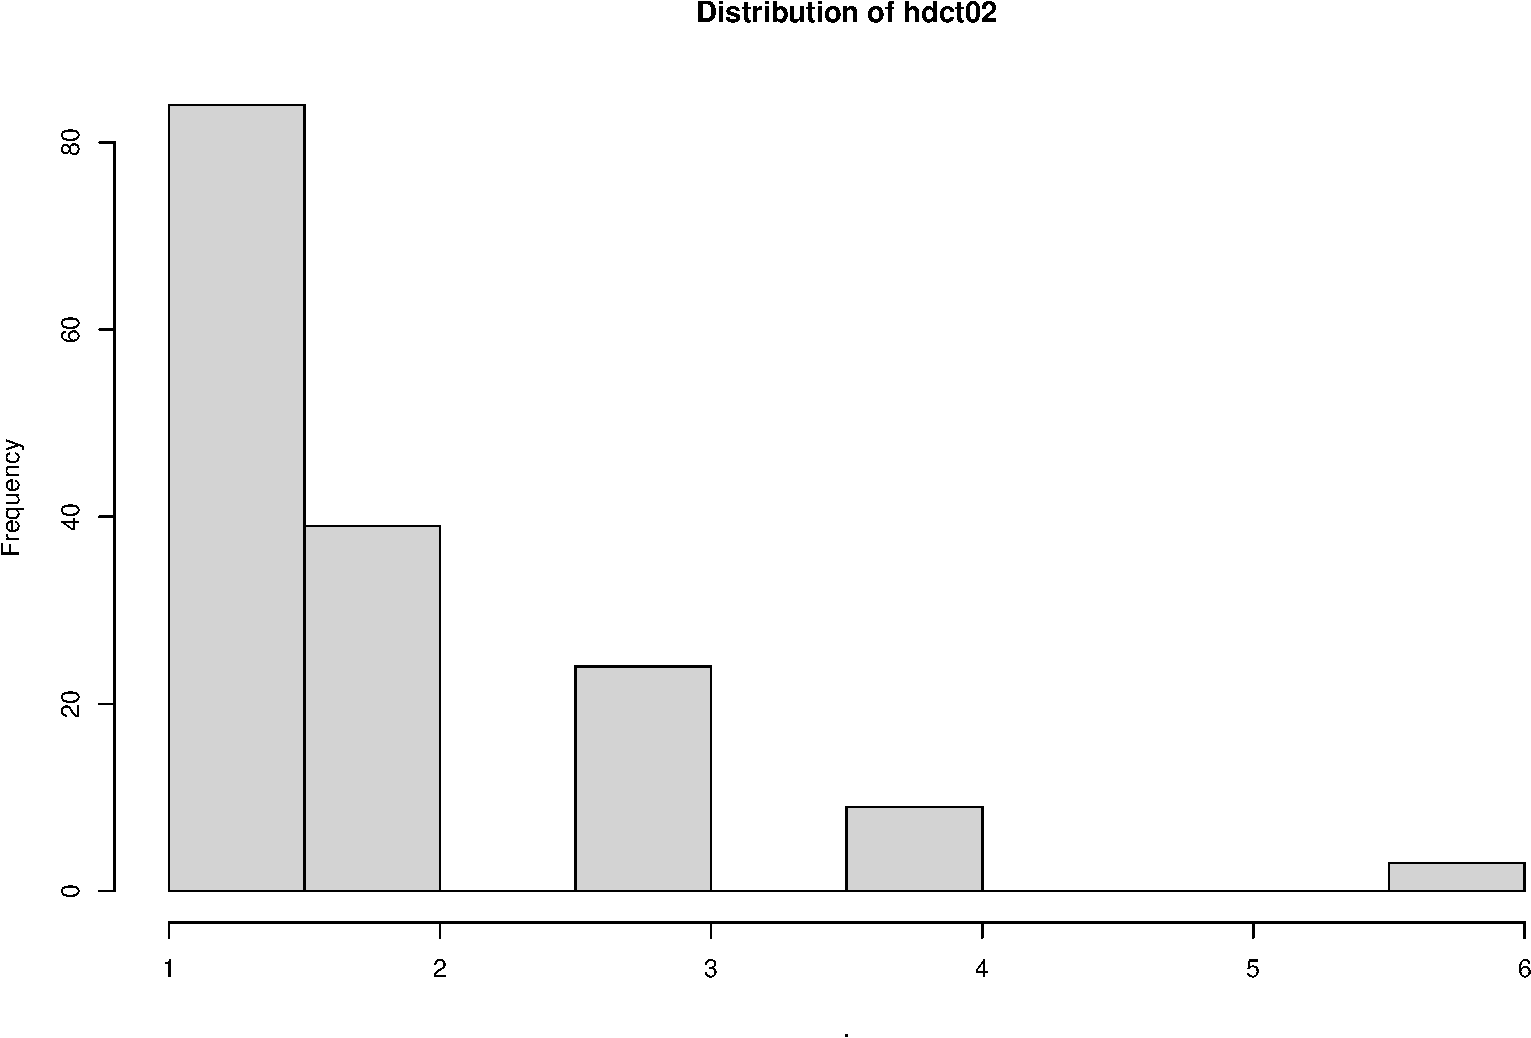
\includegraphics{week14p2_files/figure-beamer/unnamed-chunk-6-1.pdf}
\end{frame}

\begin{frame}[fragile]{}
\protect\hypertarget{section-6}{}
\tiny

\begin{Shaded}
\begin{Highlighting}[]
\NormalTok{echinacea}\SpecialCharTok{$}\NormalTok{redata }\SpecialCharTok{\%\textgreater{}\%} \FunctionTok{filter}\NormalTok{(id }\SpecialCharTok{\%in\%}\NormalTok{ (echinacea}\SpecialCharTok{$}\NormalTok{redata }\SpecialCharTok{\%\textgreater{}\%} 
                                       \FunctionTok{filter}\NormalTok{(varb }\SpecialCharTok{==} \StringTok{"fl03"} \SpecialCharTok{\&}\NormalTok{ resp }\SpecialCharTok{==} \DecValTok{1}\NormalTok{) }\SpecialCharTok{\%\textgreater{}\%} 
                                       \FunctionTok{pull}\NormalTok{(id)) }\SpecialCharTok{\&}\NormalTok{ varb }\SpecialCharTok{==} \StringTok{"hdct03"}\NormalTok{) }\SpecialCharTok{\%\textgreater{}\%} 
  \FunctionTok{pull}\NormalTok{(resp) }\SpecialCharTok{\%\textgreater{}\%} \FunctionTok{hist}\NormalTok{(., }\AttributeTok{main =} \StringTok{"Distribution of hdct03"}\NormalTok{)}
\end{Highlighting}
\end{Shaded}

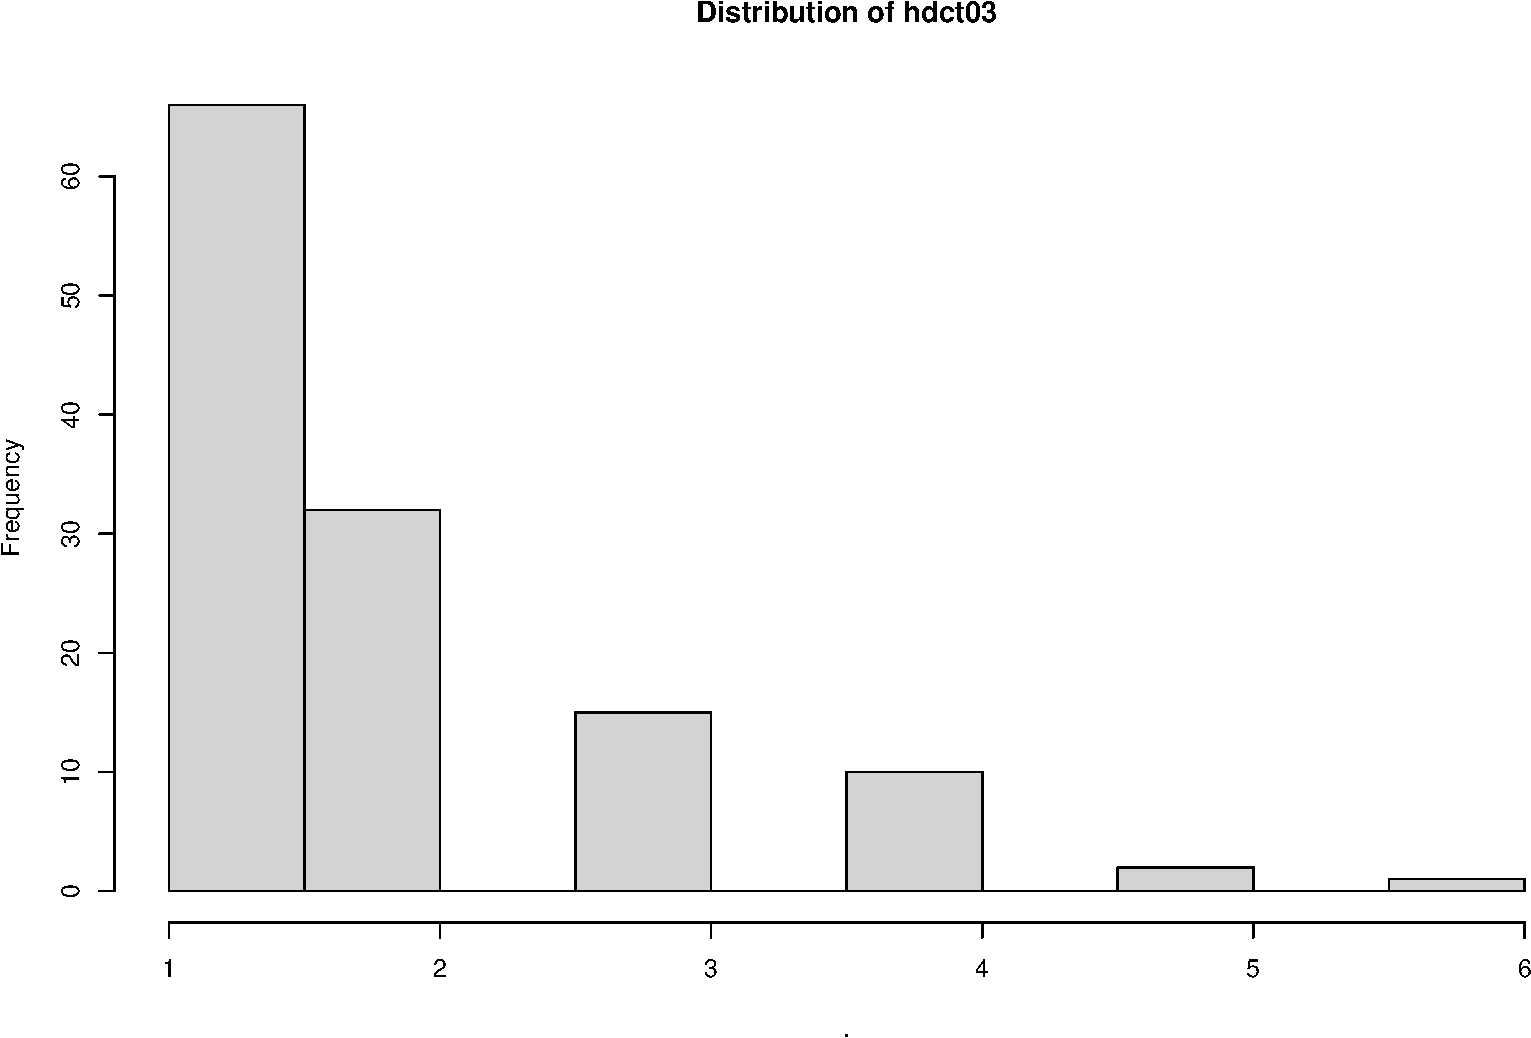
\includegraphics{week14p2_files/figure-beamer/unnamed-chunk-7-1.pdf}
\end{frame}

\begin{frame}[fragile]{}
\protect\hypertarget{section-7}{}
\tiny

\begin{Shaded}
\begin{Highlighting}[]
\NormalTok{echinacea}\SpecialCharTok{$}\NormalTok{redata }\SpecialCharTok{\%\textgreater{}\%} \FunctionTok{filter}\NormalTok{(id }\SpecialCharTok{\%in\%}\NormalTok{ (echinacea}\SpecialCharTok{$}\NormalTok{redata }\SpecialCharTok{\%\textgreater{}\%} 
                                       \FunctionTok{filter}\NormalTok{(varb }\SpecialCharTok{==} \StringTok{"fl04"} \SpecialCharTok{\&}\NormalTok{ resp }\SpecialCharTok{==} \DecValTok{1}\NormalTok{) }\SpecialCharTok{\%\textgreater{}\%} 
                                       \FunctionTok{pull}\NormalTok{(id)) }\SpecialCharTok{\&}\NormalTok{ varb }\SpecialCharTok{==} \StringTok{"hdct04"}\NormalTok{) }\SpecialCharTok{\%\textgreater{}\%} 
  \FunctionTok{pull}\NormalTok{(resp) }\SpecialCharTok{\%\textgreater{}\%} \FunctionTok{hist}\NormalTok{(., }\AttributeTok{main =} \StringTok{"Distribution of hdct04"}\NormalTok{)}
\end{Highlighting}
\end{Shaded}

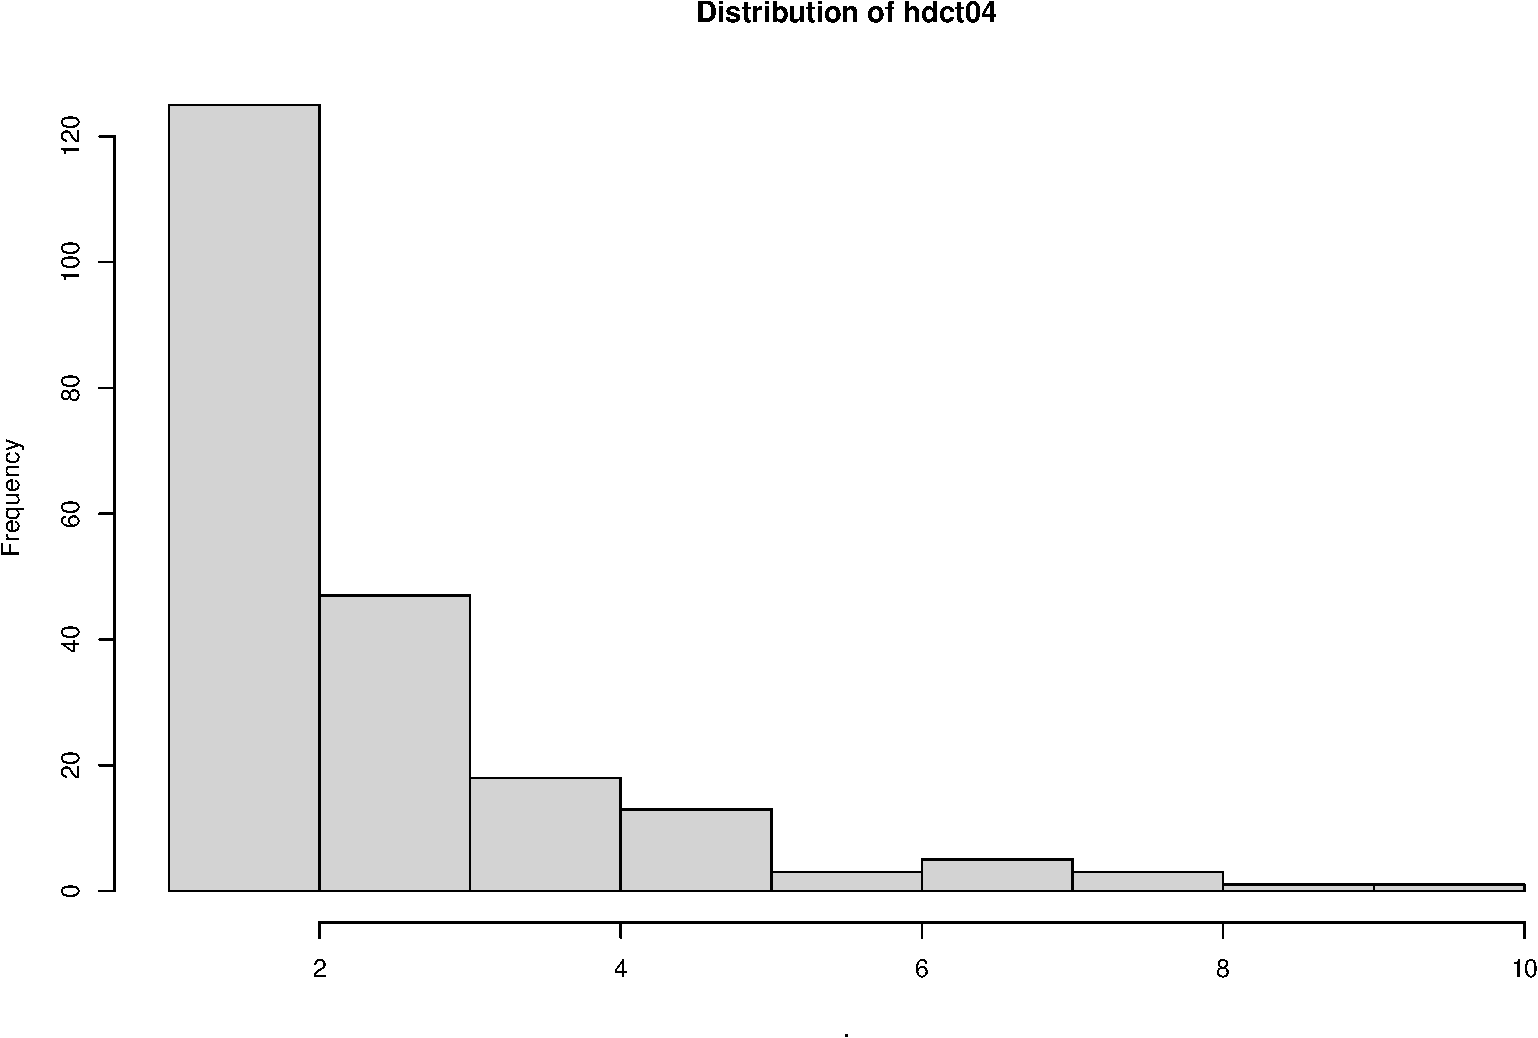
\includegraphics{week14p2_files/figure-beamer/unnamed-chunk-8-1.pdf}
\end{frame}

\begin{frame}[fragile]{}
\protect\hypertarget{section-8}{}
\tiny

\begin{Shaded}
\begin{Highlighting}[]
\NormalTok{echinacea}\SpecialCharTok{$}\NormalTok{redata }\SpecialCharTok{\%\textgreater{}\%} \FunctionTok{group\_by}\NormalTok{(id) }\SpecialCharTok{\%\textgreater{}\%} 
  \FunctionTok{filter}\NormalTok{(varb }\SpecialCharTok{\%in\%} \FunctionTok{c}\NormalTok{(}\StringTok{"hdct02"}\NormalTok{,}\StringTok{"hdct03"}\NormalTok{,}\StringTok{"hdct04"}\NormalTok{)) }\SpecialCharTok{\%\textgreater{}\%} 
  \FunctionTok{summarise}\NormalTok{(}\AttributeTok{fitness =} \FunctionTok{sum}\NormalTok{(resp)) }\SpecialCharTok{\%\textgreater{}\%} 
  \FunctionTok{pull}\NormalTok{(fitness) }\SpecialCharTok{\%\textgreater{}\%} \FunctionTok{hist}\NormalTok{(., }\AttributeTok{main =} \StringTok{"Distribution of fitness"}\NormalTok{, }\AttributeTok{breaks =} \DecValTok{20}\NormalTok{)}
\end{Highlighting}
\end{Shaded}

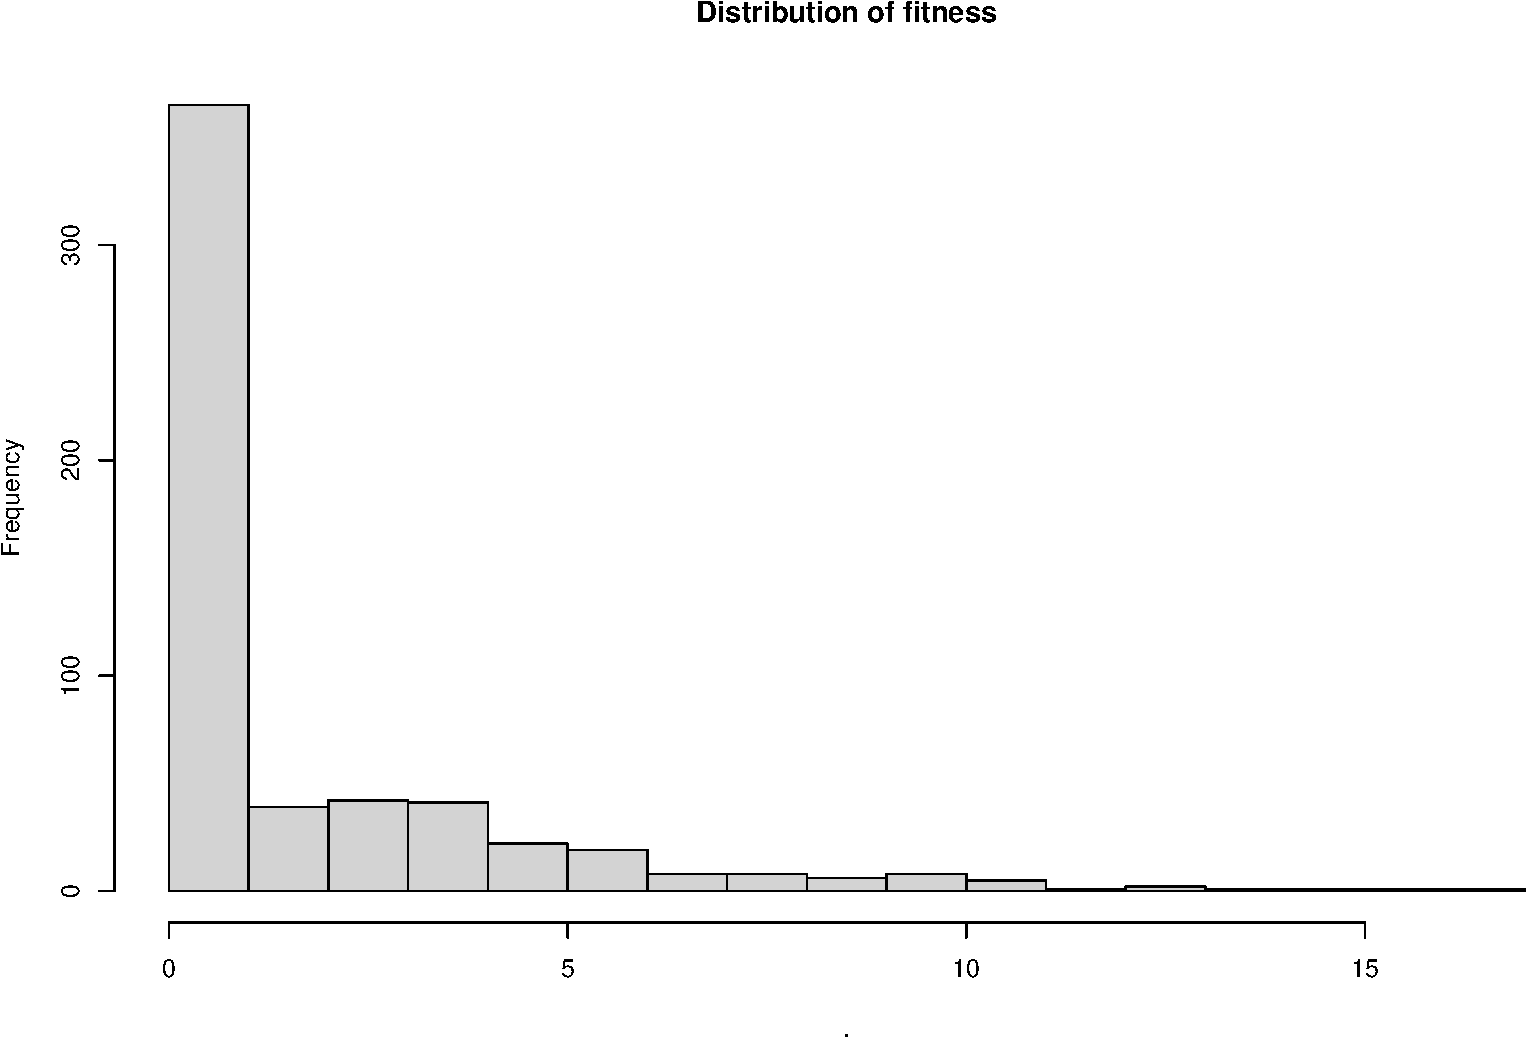
\includegraphics{week14p2_files/figure-beamer/unnamed-chunk-9-1.pdf}
\end{frame}

\begin{frame}[fragile]{Aster analysis preliminaries}
\protect\hypertarget{aster-analysis-preliminaries}{}
The variables that correspond to nodes of the graph are, in the order
they are numbered in the graph \vspace{12pt}

\begin{Shaded}
\begin{Highlighting}[]
\NormalTok{vars }\OtherTok{\textless{}{-}} \FunctionTok{c}\NormalTok{(}\StringTok{"ld02"}\NormalTok{, }\StringTok{"ld03"}\NormalTok{, }\StringTok{"ld04"}\NormalTok{, }\StringTok{"fl02"}\NormalTok{, }\StringTok{"fl03"}\NormalTok{, }
                    \StringTok{"fl04"}\NormalTok{, }\StringTok{"hdct02"}\NormalTok{, }\StringTok{"hdct03"}\NormalTok{, }\StringTok{"hdct04"}\NormalTok{)}
\end{Highlighting}
\end{Shaded}
\end{frame}

\begin{frame}[fragile]{}
\protect\hypertarget{section-9}{}
The graphical structure is specified by a vector that gives for each
node the index (not the name) of the predecessor node or zero if the
predecessor is an initial node.

\vspace{12pt}

\begin{Shaded}
\begin{Highlighting}[]
\NormalTok{pred }\OtherTok{\textless{}{-}} \FunctionTok{c}\NormalTok{(}\DecValTok{0}\NormalTok{, }\DecValTok{1}\NormalTok{, }\DecValTok{2}\NormalTok{, }\DecValTok{1}\NormalTok{, }\DecValTok{2}\NormalTok{, }\DecValTok{3}\NormalTok{, }\DecValTok{4}\NormalTok{, }\DecValTok{5}\NormalTok{, }\DecValTok{6}\NormalTok{)}
\end{Highlighting}
\end{Shaded}

\vspace{12pt}

This says the predecessor of the first node given by the \texttt{vars}
vector is initial (because \texttt{pred[1] == 0}), the predecessor of
the second node given by the \texttt{vars} vector is the first node
given by the \texttt{vars} vector (because \texttt{pred[2] == 1}), and
so forth.
\end{frame}

\begin{frame}[fragile]{}
\protect\hypertarget{section-10}{}
\tiny

\begin{Shaded}
\begin{Highlighting}[]
\NormalTok{foo }\OtherTok{\textless{}{-}} \FunctionTok{rbind}\NormalTok{(vars, }\FunctionTok{c}\NormalTok{(}\StringTok{"initial"}\NormalTok{, vars)[pred }\SpecialCharTok{+} \DecValTok{1}\NormalTok{]) }
\FunctionTok{rownames}\NormalTok{(foo) }\OtherTok{\textless{}{-}} \FunctionTok{c}\NormalTok{(}\StringTok{"successor"}\NormalTok{, }\StringTok{"predecessor"}\NormalTok{)}
\NormalTok{foo}
\end{Highlighting}
\end{Shaded}

\begin{verbatim}
##             [,1]      [,2]   [,3]   [,4]   [,5]   [,6]   [,7]     [,8]    
## successor   "ld02"    "ld03" "ld04" "fl02" "fl03" "fl04" "hdct02" "hdct03"
## predecessor "initial" "ld02" "ld03" "ld02" "ld03" "ld04" "fl02"   "fl03"  
##             [,9]    
## successor   "hdct04"
## predecessor "fl04"
\end{verbatim}

\vspace{12pt}
\normalsize

That's right.
\end{frame}

\begin{frame}{}
\protect\hypertarget{section-11}{}
The last part of the specification of the graph is given by a
corresponding vector of integers coding families (distributions). The
default is to use the codes:

\begin{itemize}
\tightlist
\item
  1 = Bernoulli
\item
  2 = Poisson
\item
  3 = zero-truncated Poisson
\end{itemize}
\end{frame}

\begin{frame}[fragile]{}
\protect\hypertarget{section-12}{}
Optionally, the integer codes specify families given by an optional
argument \texttt{famlist} to functions in the \texttt{aster} package,
and this can specify other distributions besides those in the default
coding.

\vspace{12pt}
\tiny

\begin{Shaded}
\begin{Highlighting}[]
\NormalTok{fam }\OtherTok{\textless{}{-}} \FunctionTok{c}\NormalTok{(}\DecValTok{1}\NormalTok{, }\DecValTok{1}\NormalTok{, }\DecValTok{1}\NormalTok{, }\DecValTok{1}\NormalTok{, }\DecValTok{1}\NormalTok{, }\DecValTok{1}\NormalTok{, }\DecValTok{3}\NormalTok{, }\DecValTok{3}\NormalTok{, }\DecValTok{3}\NormalTok{)}
\FunctionTok{rbind}\NormalTok{(vars, fam)}
\end{Highlighting}
\end{Shaded}

\begin{verbatim}
##      [,1]   [,2]   [,3]   [,4]   [,5]   [,6]   [,7]     [,8]     [,9]    
## vars "ld02" "ld03" "ld04" "fl02" "fl03" "fl04" "hdct02" "hdct03" "hdct04"
## fam  "1"    "1"    "1"    "1"    "1"    "1"    "3"      "3"      "3"
\end{verbatim}
\end{frame}

\begin{frame}[fragile]{}
\protect\hypertarget{section-13}{}
There is one more step before we can fit models.

The R function \texttt{aster} which fits aster models wants the data in
long rather than wide format, the former having one line per node of the
graph rather than one per individual.

\vspace{12pt}
\tiny

\begin{Shaded}
\begin{Highlighting}[]
\DocumentationTok{\#\# aster example already in long format}
\NormalTok{redata }\OtherTok{\textless{}{-}} \FunctionTok{data.frame}\NormalTok{(echinacea}\SpecialCharTok{$}\NormalTok{redata, }\AttributeTok{root =} \DecValTok{1}\NormalTok{)}
\FunctionTok{head}\NormalTok{(redata)}
\end{Highlighting}
\end{Shaded}

\begin{verbatim}
##           pop ewloc nsloc varb resp id root
## 1.ld02   NWLF    -8   -11 ld02    0  1    1
## 2.ld02 Eriley    -8   -10 ld02    1  2    1
## 3.ld02   NWLF    -8    -9 ld02    0  3    1
## 4.ld02    SPP    -8    -8 ld02    0  4    1
## 5.ld02    SPP    -8    -7 ld02    0  5    1
## 6.ld02 Eriley    -8    -6 ld02    1  6    1
\end{verbatim}
\end{frame}

\begin{frame}[fragile]{}
\protect\hypertarget{section-14}{}
All of the variables in \texttt{echinacea} that are named in
\texttt{vars} are gone. They are packed into the variable \texttt{resp}.

Which components of \texttt{resp} correspond to which components of
\texttt{vars} is shown by the new variable \texttt{varb}.

\vspace{12pt}
\tiny

\begin{Shaded}
\begin{Highlighting}[]
\FunctionTok{levels}\NormalTok{(redata}\SpecialCharTok{$}\NormalTok{varb)}
\end{Highlighting}
\end{Shaded}

\begin{verbatim}
## [1] "ld02"   "ld03"   "ld04"   "fl02"   "fl03"   "fl04"   "hdct02" "hdct03"
## [9] "hdct04"
\end{verbatim}
\end{frame}

\begin{frame}{Fitting aster models}
\protect\hypertarget{fitting-aster-models}{}
We will now discuss fitting aster models.

Different families for different nodes of the graph means it makes no
sense to have terms of the regression formula applying to different
nodes.

In particular, it makes no sense to have one \emph{intercept} for all
nodes. To in effect get a different \emph{intercept} for each node in
the graph, include \texttt{varb} in the formula

\begin{center}
  \texttt{y $\sim$ varb + ...}
\end{center}

The categorical variable \texttt{varb} gets turned into as many dummy
variables as there are nodes in the graph, one is dropped, and the
\emph{intercept} dummy variable.
\end{frame}

\begin{frame}{}
\protect\hypertarget{section-15}{}
Similar thinking says we want completely different regression
coefficients of all kinds of predictors for each node of the graph.

That would lead us to formulas like

\begin{center}
  \texttt{y $\sim$ varb + varb:(...)}
\end{center}

where \(\ldots\) is any other part of the formula.

We should not think of this formula as specifying \emph{interaction}
between \texttt{varb} and terms in the model but rather as specifying
separate coefficients for the terms in the model for each node of the
graph.

That being said, formulas like this would likely yield too many
regression coefficients to estimate well.
\end{frame}

\begin{frame}[fragile]{}
\protect\hypertarget{section-16}{}
Maybe different coefficients for each kind of node (ie mortality or head
count) would be good enough.

\vspace{12pt}
\tiny

\begin{Shaded}
\begin{Highlighting}[]
\NormalTok{layer }\OtherTok{\textless{}{-}} \FunctionTok{gsub}\NormalTok{(}\StringTok{"[0{-}9]"}\NormalTok{, }\StringTok{""}\NormalTok{, }\FunctionTok{as.character}\NormalTok{(redata}\SpecialCharTok{$}\NormalTok{varb))}
\NormalTok{redata }\OtherTok{\textless{}{-}} \FunctionTok{data.frame}\NormalTok{(redata, }\AttributeTok{layer =}\NormalTok{ layer)}
\FunctionTok{unique}\NormalTok{(layer)}
\end{Highlighting}
\end{Shaded}

\begin{verbatim}
## [1] "ld"   "fl"   "hdct"
\end{verbatim}

\vspace{12pt}
\normalsize

Maybe

\begin{center}
  \texttt{y $\sim$ varb + layer:(...)}
\end{center}

is good enough? But formulas like this would still yield too many
regression coefficients to estimate well.
\end{frame}

\begin{frame}[fragile]{}
\protect\hypertarget{section-17}{}
In aster models regression coefficients \emph{for} a node of the graph
also influence all \emph{earlier} nodes of the graph (predecessor,
predecessor of predecessor, predecessor of predecessor of predecessor,
etc.)

So maybe it would be good enough to only have separate coefficients for
the layer of the graph consisting of terminal nodes?

\vspace{12pt}

\begin{Shaded}
\begin{Highlighting}[]
\NormalTok{fit }\OtherTok{\textless{}{-}} \FunctionTok{as.numeric}\NormalTok{(layer }\SpecialCharTok{==} \StringTok{"hdct"}\NormalTok{) }
\NormalTok{redata }\OtherTok{\textless{}{-}} \FunctionTok{data.frame}\NormalTok{(redata, }\AttributeTok{fit =}\NormalTok{ fit)}
\FunctionTok{unique}\NormalTok{(fit)}
\end{Highlighting}
\end{Shaded}

\begin{verbatim}
## [1] 0 1
\end{verbatim}
\end{frame}

\begin{frame}{}
\protect\hypertarget{section-18}{}
Maybe

\begin{center}
  \texttt{y $\sim$ varb + fit:(...)}
\end{center}

is good enough.

We called the variable we just made up \texttt{fit} which is short for
Darwinian fitness.

The regression coefficients in terms specified by \(\ldots\) have a
direct relationship with expected Darwinian fitness (or a surrogate of
Darwinian fitness).

And that is usually what is wanted in life history analysis.
\end{frame}

\begin{frame}[fragile]{}
\protect\hypertarget{section-19}{}
We now fit our first aster model.

\vspace{12pt}
\tiny

\begin{Shaded}
\begin{Highlighting}[]
\NormalTok{aout }\OtherTok{\textless{}{-}} \FunctionTok{aster}\NormalTok{(resp }\SpecialCharTok{\textasciitilde{}}\NormalTok{ varb }\SpecialCharTok{+}\NormalTok{ layer }\SpecialCharTok{:}\NormalTok{ (nsloc }\SpecialCharTok{+}\NormalTok{ ewloc) }\SpecialCharTok{+} 
\NormalTok{                            fit }\SpecialCharTok{:}\NormalTok{ pop, pred, fam, varb, id, root, }\AttributeTok{data =}\NormalTok{ redata)}
\FunctionTok{summary}\NormalTok{(aout)}
\end{Highlighting}
\end{Shaded}

\begin{verbatim}
## 
## Call:
## aster.formula(formula = resp ~ varb + layer:(nsloc + ewloc) + 
##     fit:pop, pred = pred, fam = fam, varvar = varb, idvar = id, 
##     root = root, data = redata)
## 
##                  Estimate Std. Error z value Pr(>|z|)    
## (Intercept)     -1.079946   0.241164  -4.478 7.53e-06 ***
## varbld03         1.769353   0.529200   3.343 0.000827 ***
## varbld04         4.217879   0.368282  11.453  < 2e-16 ***
## varbfl02         0.029302   0.315703   0.093 0.926050    
## varbfl03        -0.319794   0.316120  -1.012 0.311720    
## varbfl04        -0.314920   0.295018  -1.067 0.285763    
## varbhdct02       1.350716   0.259254   5.210 1.89e-07 ***
## varbhdct03       1.372676   0.262255   5.234 1.66e-07 ***
## varbhdct04       1.880630   0.251000   7.493 6.75e-14 ***
## layerfl:nsloc    0.070102   0.014652   4.785 1.71e-06 ***
## layerhdct:nsloc -0.005804   0.005550  -1.046 0.295638    
## layerld:nsloc    0.007165   0.005867   1.221 0.221957    
## layerfl:ewloc    0.017977   0.014413   1.247 0.212294    
## layerhdct:ewloc  0.007606   0.005561   1.368 0.171381    
## layerld:ewloc   -0.004787   0.005919  -0.809 0.418635    
## fit:popAA        0.129238   0.089129   1.450 0.147058    
## fit:popEriley   -0.049561   0.071279  -0.695 0.486858    
## fit:popLf       -0.033279   0.079573  -0.418 0.675789    
## fit:popNessman  -0.186269   0.127787  -1.458 0.144936    
## fit:popNWLF      0.021028   0.063600   0.331 0.740920    
## fit:popSPP       0.149179   0.067716   2.203 0.027593 *  
## ---
## Signif. codes:  0 '***' 0.001 '**' 0.01 '*' 0.05 '.' 0.1 ' ' 1
## 
## Original predictor variables dropped (aliased)
##      fit:popStevens
\end{verbatim}
\end{frame}

\begin{frame}[fragile]{}
\protect\hypertarget{section-20}{}
The regression coefficients are of little interest.

The main interest is in what model among those that have a scientific
interpretation fits the best.

\vspace{12pt}
\tiny

\begin{Shaded}
\begin{Highlighting}[]
\NormalTok{aout.smaller }\OtherTok{\textless{}{-}} \FunctionTok{aster}\NormalTok{(resp }\SpecialCharTok{\textasciitilde{}}\NormalTok{ varb }\SpecialCharTok{+} 
\NormalTok{  fit }\SpecialCharTok{:}\NormalTok{ (nsloc }\SpecialCharTok{+}\NormalTok{ ewloc }\SpecialCharTok{+}\NormalTok{ pop), }
\NormalTok{  pred, fam, varb, id, root, }\AttributeTok{data =}\NormalTok{ redata)}
\NormalTok{aout.bigger }\OtherTok{\textless{}{-}} \FunctionTok{aster}\NormalTok{(resp }\SpecialCharTok{\textasciitilde{}}\NormalTok{ varb }\SpecialCharTok{+} 
\NormalTok{  layer }\SpecialCharTok{:}\NormalTok{ (nsloc }\SpecialCharTok{+}\NormalTok{ ewloc }\SpecialCharTok{+}\NormalTok{ pop), }
\NormalTok{  pred, fam, varb, id, root, }\AttributeTok{data =}\NormalTok{ redata)}
\FunctionTok{anova}\NormalTok{(aout.smaller, aout, aout.bigger)}
\end{Highlighting}
\end{Shaded}

\begin{verbatim}
## Analysis of Deviance Table
## 
## Model 1: resp ~ varb + fit:(nsloc + ewloc + pop)
## Model 2: resp ~ varb + layer:(nsloc + ewloc) + fit:pop
## Model 3: resp ~ varb + layer:(nsloc + ewloc + pop)
##   Model Df Model Dev Df Deviance P(>|Chi|)    
## 1       17   -2746.7                          
## 2       21   -2712.5  4   34.203 6.772e-07 ***
## 3       33   -2674.7 12   37.838 0.0001632 ***
## ---
## Signif. codes:  0 '***' 0.001 '**' 0.01 '*' 0.05 '.' 0.1 ' ' 1
\end{verbatim}
\end{frame}

\begin{frame}{}
\protect\hypertarget{section-21}{}
Despite the largest model fitting the best, we choose the middle model
because that one tells us something about fitness directly that the
other one does not.

The argument for doing this is because we are interested in modeling
fitness, and the distribution of fitness (actually best surrogate of
fitness in their data) is not very different between the two models.

The distribution of other components of fitness (other than the final
one) may differ quite a lot, but that was not the question of scientific
interest.
\end{frame}

\begin{frame}[fragile]{}
\protect\hypertarget{section-22}{}
So what do these models say about the distribution of fitness?

\vspace{12pt}
\tiny

\begin{Shaded}
\begin{Highlighting}[]
\DocumentationTok{\#\# we will go over this later}
\NormalTok{pop }\OtherTok{\textless{}{-}} \FunctionTok{levels}\NormalTok{(redata}\SpecialCharTok{$}\NormalTok{pop)}
\NormalTok{nind }\OtherTok{\textless{}{-}} \FunctionTok{length}\NormalTok{(}\FunctionTok{unique}\NormalTok{(redata}\SpecialCharTok{$}\NormalTok{id))}
\NormalTok{nnode }\OtherTok{\textless{}{-}} \FunctionTok{nlevels}\NormalTok{(redata}\SpecialCharTok{$}\NormalTok{varb)}
\NormalTok{npop }\OtherTok{\textless{}{-}} \FunctionTok{length}\NormalTok{(pop)}
\NormalTok{amat }\OtherTok{\textless{}{-}} \FunctionTok{array}\NormalTok{(}\DecValTok{0}\NormalTok{, }\FunctionTok{c}\NormalTok{(nind, nnode, npop))}
\NormalTok{amat.ind }\OtherTok{\textless{}{-}} \FunctionTok{array}\NormalTok{(}\FunctionTok{as.character}\NormalTok{(redata}\SpecialCharTok{$}\NormalTok{pop), }
  \FunctionTok{c}\NormalTok{(nind, nnode, npop))}
\NormalTok{amat.node }\OtherTok{\textless{}{-}} \FunctionTok{array}\NormalTok{(}\FunctionTok{as.character}\NormalTok{(redata}\SpecialCharTok{$}\NormalTok{varb), }
  \FunctionTok{c}\NormalTok{(nind, nnode, npop))}
\NormalTok{amat.fit }\OtherTok{\textless{}{-}} \FunctionTok{grepl}\NormalTok{(}\StringTok{"hdct"}\NormalTok{, amat.node)}
\NormalTok{amat.fit }\OtherTok{\textless{}{-}} \FunctionTok{array}\NormalTok{(amat.fit, }
  \FunctionTok{c}\NormalTok{(nind, nnode, npop))}
\NormalTok{amat.pop }\OtherTok{\textless{}{-}} \FunctionTok{array}\NormalTok{(pop, }\FunctionTok{c}\NormalTok{(npop, nnode, nind))}
\NormalTok{amat.pop }\OtherTok{\textless{}{-}} \FunctionTok{aperm}\NormalTok{(amat.pop)}
\NormalTok{amat[amat.pop }\SpecialCharTok{==}\NormalTok{ amat.ind }\SpecialCharTok{\&}\NormalTok{ amat.fit] }\OtherTok{\textless{}{-}} \DecValTok{1}
\NormalTok{pout }\OtherTok{\textless{}{-}} \FunctionTok{predict}\NormalTok{(aout,  }\AttributeTok{varvar =}\NormalTok{ varb, }\AttributeTok{idvar =}\NormalTok{ id, }
  \AttributeTok{root =}\NormalTok{ root, }\AttributeTok{se.fit =} \ConstantTok{TRUE}\NormalTok{, }\AttributeTok{amat =}\NormalTok{ amat)}
\NormalTok{pout.bigger }\OtherTok{\textless{}{-}} \FunctionTok{predict}\NormalTok{(aout.bigger, }\AttributeTok{varvar =}\NormalTok{ varb, }
  \AttributeTok{idvar =}\NormalTok{ id, }\AttributeTok{root =}\NormalTok{ root, }\AttributeTok{se.fit =} \ConstantTok{TRUE}\NormalTok{, }\AttributeTok{amat =}\NormalTok{ amat)}
\end{Highlighting}
\end{Shaded}
\end{frame}

\begin{frame}[fragile]{}
\protect\hypertarget{section-23}{}
The first interesting thing about these \emph{predictions} (actually
point estimates of parameters with standard errors) is that the point
estimates are exactly the same for the two models.

\vspace{12pt}
\tiny

\begin{Shaded}
\begin{Highlighting}[]
\NormalTok{pout}\SpecialCharTok{$}\NormalTok{fit}
\end{Highlighting}
\end{Shaded}

\begin{verbatim}
## [1]  81 171 112  31 286 218 167
\end{verbatim}

\begin{Shaded}
\begin{Highlighting}[]
\NormalTok{pout.bigger}\SpecialCharTok{$}\NormalTok{fit}
\end{Highlighting}
\end{Shaded}

\begin{verbatim}
## [1]  81 171 112  31 286 218 167
\end{verbatim}

\begin{Shaded}
\begin{Highlighting}[]
\FunctionTok{all.equal}\NormalTok{(pout}\SpecialCharTok{$}\NormalTok{fit, pout.bigger}\SpecialCharTok{$}\NormalTok{fit)}
\end{Highlighting}
\end{Shaded}

\begin{verbatim}
## [1] TRUE
\end{verbatim}

\vspace{12pt}
\normalsize

And why is that? These are submodel canonical statistics (components of
\(M^Ty\)). Thus by the observed-equals-expected property of exponential
families their MLE are equal to their observed values and hence equal to
each other.

So that is certainly not a reason to prefer one model to the other. If
the estimated means are exactly the same how about estimated asymptotic
variances?
\end{frame}

\begin{frame}[fragile]{}
\protect\hypertarget{section-24}{}
The asymptotic variance matrix of these canonical statistics is actually
diagonal for each model.

The reason is that different populations of origin have different
individuals in the sample, and only individuals from one population
contribute to estimating one of these canonical statistics.

Thus it is enough to look at the asymptotic standard errors (all the
covariances are zero).

\vspace{12pt}
\tiny

\begin{Shaded}
\begin{Highlighting}[]
\NormalTok{pout}\SpecialCharTok{$}\NormalTok{se.fit}
\end{Highlighting}
\end{Shaded}

\begin{verbatim}
## [1] 13.617532 19.984170 16.267065  8.524453 25.968492 22.227096 19.884556
\end{verbatim}

\begin{Shaded}
\begin{Highlighting}[]
\NormalTok{pout.bigger}\SpecialCharTok{$}\NormalTok{se.fit}
\end{Highlighting}
\end{Shaded}

\begin{verbatim}
## [1] 14.521691 17.870387 14.513433  9.105173 27.857509 21.589790 21.642168
\end{verbatim}

\vspace{12pt}
\normalsize

We see that they are not that different.
\end{frame}

\begin{frame}{}
\protect\hypertarget{section-25}{}
If we were interested in the effect of population on the different
components of fitness, then the P-value 0.00016 does indicate that the
model \texttt{aout.bigger} fits the data better.

The model \texttt{aout.bigger} has different population effects in
different \emph{layers} of the graph does show a statistically
significant difference in the way the components of fitness combine to
make up fitness in the various population of origin groups.

But if we are only interested in overall fitness rather than the
separate components, then there is hardly any difference in the two
models.
\end{frame}

\begin{frame}{Estimating expected Darwinian fitness}
\protect\hypertarget{estimating-expected-darwinian-fitness}{}
Hypothesis tests using the R function \texttt{anova} are fairly
straightforward.

Confidence intervals using the R function \texttt{predict} for estimates
of expected Darwinian fitness are anything but straightforward.

Among other issues, aster models have six different parameterizations,
all of which can be of scientific interest in some applications.
\end{frame}

\begin{frame}{}
\protect\hypertarget{section-26}{}
\begin{center}
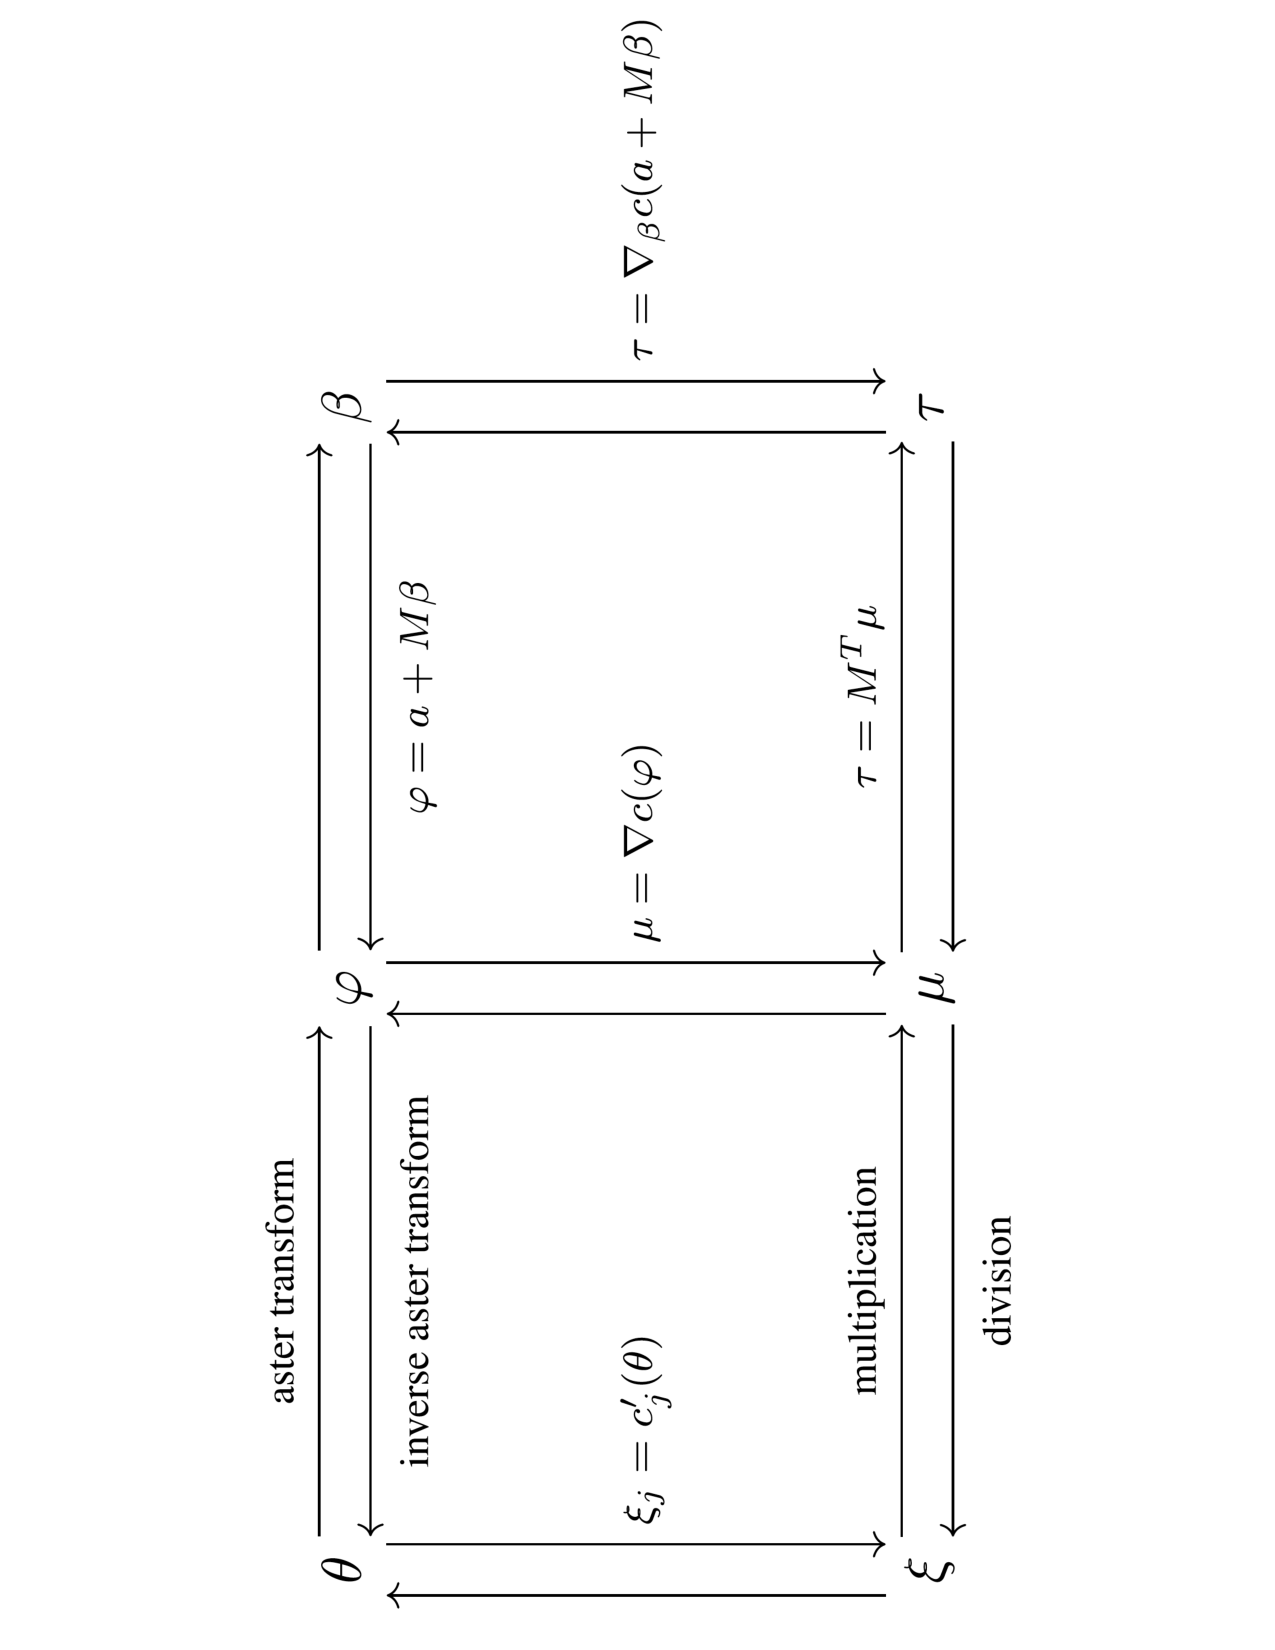
\includegraphics[angle=270, width=0.75\textwidth]{transforms.pdf}
\end{center}
\end{frame}

\begin{frame}[fragile]{}
\protect\hypertarget{section-27}{}
The result of \texttt{predict(aout)} is the maximum likelihood estimate
of the saturated model mean value parameter vector \(\mu\).

If we want to say how bad or good our estimators are, then we need
confidence intervals (or perhaps just standard errors).

\vspace{12pt}
\tiny

\begin{Shaded}
\begin{Highlighting}[]
\NormalTok{pout }\OtherTok{\textless{}{-}} \FunctionTok{predict}\NormalTok{(aout, }\AttributeTok{se.fit =} \ConstantTok{TRUE}\NormalTok{)}
\end{Highlighting}
\end{Shaded}

\vspace{12pt}
\normalsize

The components of \texttt{predict(aout)} are

\begin{itemize}
  \item The component \texttt{fit} gives the estimators (the same vector that was returned when predict was invoked with no optional arguments).
  \item The component \texttt{se.fit} gives the corresponding standard errors.
  \item The component \texttt{gradient} gives the derivative of the map from regression coefficients to predictions.
\end{itemize}
\end{frame}

\begin{frame}{}
\protect\hypertarget{section-28}{}
These are asymptotic (large sample size, approximate) estimated standard
deviations of the components of \(\hat\mu\) derived using the usual
theory of maximum likelihood estimation.

In any event, suppose the parameter of interest is given by
\(h(\beta)\). Then this parameter has an estimator with the following
asymptotic distribution \[
  \sqrt{n}(h(\hat\beta) - h(\beta)) \to N\left(0, \nabla h(\beta)\Sigma^{-1} \{\nabla h(\beta)\}^T \right).
\]
\end{frame}

\begin{frame}[fragile]{}
\protect\hypertarget{section-29}{}
Below are confidence bounds for approximate 95\% confidence intervals
(not corrected for simultaneous coverage) for each of the components of
the response vector.

\vspace{12pt}
\tiny

\begin{Shaded}
\begin{Highlighting}[]
\NormalTok{low }\OtherTok{\textless{}{-}}\NormalTok{ pout}\SpecialCharTok{$}\NormalTok{fit }\SpecialCharTok{{-}} \FunctionTok{qnorm}\NormalTok{(}\FloatTok{0.975}\NormalTok{) }\SpecialCharTok{*}\NormalTok{ pout}\SpecialCharTok{$}\NormalTok{se.fit}
\NormalTok{hig }\OtherTok{\textless{}{-}}\NormalTok{ pout}\SpecialCharTok{$}\NormalTok{fit }\SpecialCharTok{+} \FunctionTok{qnorm}\NormalTok{(}\FloatTok{0.975}\NormalTok{) }\SpecialCharTok{*}\NormalTok{ pout}\SpecialCharTok{$}\NormalTok{se.fit}
\end{Highlighting}
\end{Shaded}

\vspace{12pt}
\normalsize

These are of no scientific interest whatsoever. The question of
scientific interest addressed by confidence intervals was about (best
surrogate of) fitness of a \emph{typical} individual in each population.
Thus we only want

\vspace{12pt}
\tiny

\begin{Shaded}
\begin{Highlighting}[]
\FunctionTok{nlevels}\NormalTok{(redata}\SpecialCharTok{$}\NormalTok{pop)}
\end{Highlighting}
\end{Shaded}

\begin{verbatim}
## [1] 7
\end{verbatim}

\vspace{12pt}
\normalsize

confidence intervals, one for each population. What do we mean by
\emph{typical} individuals?
\end{frame}

\begin{frame}[fragile]{}
\protect\hypertarget{section-30}{}
Those that are directly comparable. Those that the same in all respects
except for population.

Thus we have to make up covariate data for hypothetical individuals that
are comparable like this and get estimated mean values for them.

\vspace{12pt}
\tiny

\begin{Shaded}
\begin{Highlighting}[]
\NormalTok{dat }\OtherTok{\textless{}{-}} \FunctionTok{data.frame}\NormalTok{(}\AttributeTok{nsloc =} \DecValTok{0}\NormalTok{, }\AttributeTok{ewloc =} \DecValTok{0}\NormalTok{, }\AttributeTok{pop =} \FunctionTok{levels}\NormalTok{(redata}\SpecialCharTok{$}\NormalTok{pop), }
  \AttributeTok{root =} \DecValTok{1}\NormalTok{, }\AttributeTok{ld02 =} \DecValTok{1}\NormalTok{, }\AttributeTok{ld03 =} \DecValTok{1}\NormalTok{, }\AttributeTok{ld04 =} \DecValTok{1}\NormalTok{, }\AttributeTok{fl02 =} \DecValTok{1}\NormalTok{, }\AttributeTok{fl03 =} \DecValTok{1}\NormalTok{, }
  \AttributeTok{fl04 =} \DecValTok{1}\NormalTok{, }\AttributeTok{hdct02 =} \DecValTok{1}\NormalTok{, }\AttributeTok{hdct03 =} \DecValTok{1}\NormalTok{, }\AttributeTok{hdct04 =} \DecValTok{1}\NormalTok{)}
\NormalTok{dat}
\end{Highlighting}
\end{Shaded}

\begin{verbatim}
##   nsloc ewloc     pop root ld02 ld03 ld04 fl02 fl03 fl04 hdct02 hdct03 hdct04
## 1     0     0      AA    1    1    1    1    1    1    1      1      1      1
## 2     0     0  Eriley    1    1    1    1    1    1    1      1      1      1
## 3     0     0      Lf    1    1    1    1    1    1    1      1      1      1
## 4     0     0 Nessman    1    1    1    1    1    1    1      1      1      1
## 5     0     0    NWLF    1    1    1    1    1    1    1      1      1      1
## 6     0     0     SPP    1    1    1    1    1    1    1      1      1      1
## 7     0     0 Stevens    1    1    1    1    1    1    1      1      1      1
\end{verbatim}
\end{frame}

\begin{frame}[fragile]{}
\protect\hypertarget{section-31}{}
The components of the response vector are ignored in prediction so we
can give them arbitrary values. Somewhat annoyingly, they have to be
possible values because \texttt{predict.aster.formula} will check.

We now wrangle this new data into a format to be used by
\texttt{predict.aster}.

\tiny
\vspace{12pt}

\begin{Shaded}
\begin{Highlighting}[]
\NormalTok{renewdata }\OtherTok{\textless{}{-}} \FunctionTok{reshape}\NormalTok{(dat, }\AttributeTok{varying =} \FunctionTok{list}\NormalTok{(vars), }
  \AttributeTok{direction =} \StringTok{"long"}\NormalTok{, }\AttributeTok{timevar =} \StringTok{"varb"}\NormalTok{, }\AttributeTok{times =} \FunctionTok{as.factor}\NormalTok{(vars), }
  \AttributeTok{v.names =} \StringTok{"resp"}\NormalTok{)}
\NormalTok{layer }\OtherTok{\textless{}{-}} \FunctionTok{gsub}\NormalTok{(}\StringTok{"[0{-}9]"}\NormalTok{, }\StringTok{""}\NormalTok{, }\FunctionTok{as.character}\NormalTok{(renewdata}\SpecialCharTok{$}\NormalTok{varb))}
\NormalTok{renewdata }\OtherTok{\textless{}{-}} \FunctionTok{data.frame}\NormalTok{(renewdata, }\AttributeTok{layer =}\NormalTok{ layer)}
\NormalTok{fit }\OtherTok{\textless{}{-}} \FunctionTok{as.numeric}\NormalTok{(layer }\SpecialCharTok{==} \StringTok{"hdct"}\NormalTok{)}
\NormalTok{renewdata }\OtherTok{\textless{}{-}} \FunctionTok{data.frame}\NormalTok{(renewdata, }\AttributeTok{fit =}\NormalTok{ fit)}
\FunctionTok{head}\NormalTok{(renewdata)}
\end{Highlighting}
\end{Shaded}

\begin{verbatim}
##        nsloc ewloc     pop root varb resp id layer fit
## 1.ld02     0     0      AA    1 ld02    1  1    ld   0
## 2.ld02     0     0  Eriley    1 ld02    1  2    ld   0
## 3.ld02     0     0      Lf    1 ld02    1  3    ld   0
## 4.ld02     0     0 Nessman    1 ld02    1  4    ld   0
## 5.ld02     0     0    NWLF    1 ld02    1  5    ld   0
## 6.ld02     0     0     SPP    1 ld02    1  6    ld   0
\end{verbatim}
\end{frame}

\begin{frame}[fragile]{}
\protect\hypertarget{section-32}{}
Now we have predictions for these variables

\vspace{12pt}
\tiny

\begin{Shaded}
\begin{Highlighting}[]
\FunctionTok{names}\NormalTok{(renewdata)}
\end{Highlighting}
\end{Shaded}

\begin{verbatim}
## [1] "nsloc" "ewloc" "pop"   "root"  "varb"  "resp"  "id"    "layer" "fit"
\end{verbatim}

\begin{Shaded}
\begin{Highlighting}[]
\NormalTok{pout }\OtherTok{\textless{}{-}} \FunctionTok{predict}\NormalTok{(aout, }\AttributeTok{newdata =}\NormalTok{ renewdata, }\AttributeTok{varvar =}\NormalTok{ varb, }
  \AttributeTok{idvar =}\NormalTok{ id, }\AttributeTok{root =}\NormalTok{ root, }\AttributeTok{se.fit =} \ConstantTok{TRUE}\NormalTok{)}
\FunctionTok{sapply}\NormalTok{(pout, length)}
\end{Highlighting}
\end{Shaded}

\begin{verbatim}
##      fit   se.fit gradient   modmat 
##       63       63     1323     1323
\end{verbatim}

\vspace{12pt}
\normalsize

Why do we need the arguments \texttt{varvar}, \texttt{idvar}, and
\texttt{root} when we did not before? More bad design (Charlie Geyer's
words, not mine).
\end{frame}

\begin{frame}{}
\protect\hypertarget{section-33}{}
So now we can make 63 not corrected for simultaneous coverage confidence
intervals, one for each of the 9 nodes of the graph for each of these 7
hypothetical individuals (one per population). These too are of no
scientific interest whatsoever. But we are getting closer.

What is of scientific interest is confidence intervals for Darwinian
fitness for these 7 individuals. Fitness (best surrogate of) in these
data is the lifetime headcount which is

\begin{center}
  \texttt{hdct02 + hdct03 + hdct04}
\end{center}

The effects of other components of fitness is already counted in head
count. You cannot have nonzero head count if you are dead or if you had
no flowers, so that is already accounted for.
\end{frame}

\begin{frame}[fragile]{}
\protect\hypertarget{section-34}{}
We now obtain estimates of \(\mu\) for each hypothetical individual,
different rows for different individuals.

\vspace{12pt}
\tiny

\begin{Shaded}
\begin{Highlighting}[]
\NormalTok{nnode }\OtherTok{\textless{}{-}} \FunctionTok{length}\NormalTok{(vars)}
\NormalTok{preds }\OtherTok{\textless{}{-}} \FunctionTok{matrix}\NormalTok{(pout}\SpecialCharTok{$}\NormalTok{fit, }\AttributeTok{ncol =}\NormalTok{ nnode) }
\FunctionTok{dim}\NormalTok{(preds)}
\end{Highlighting}
\end{Shaded}

\begin{verbatim}
## [1] 7 9
\end{verbatim}

\begin{Shaded}
\begin{Highlighting}[]
\FunctionTok{rownames}\NormalTok{(preds) }\OtherTok{\textless{}{-}} \FunctionTok{unique}\NormalTok{(}\FunctionTok{as.character}\NormalTok{(renewdata}\SpecialCharTok{$}\NormalTok{pop))}
\FunctionTok{colnames}\NormalTok{(preds) }\OtherTok{\textless{}{-}} \FunctionTok{unique}\NormalTok{(}\FunctionTok{as.character}\NormalTok{(renewdata}\SpecialCharTok{$}\NormalTok{varb))}
\NormalTok{preds}
\end{Highlighting}
\end{Shaded}

\begin{verbatim}
##              ld02      ld03      ld04      fl02      fl03      fl04    hdct02
## AA      0.7833884 0.7521016 0.7284738 0.3228949 0.2560121 0.4560906 0.6215239
## Eriley  0.6954310 0.6565099 0.6299422 0.2333911 0.1774180 0.3236674 0.4084934
## Lf      0.7029431 0.6646121 0.6382397 0.2404182 0.1834251 0.3342160 0.4242352
## Nessman 0.6377067 0.5946209 0.5668688 0.1824325 0.1347627 0.2469403 0.2993480
## NWLF    0.7288502 0.6926410 0.6670184 0.2654522 0.2050578 0.3716382 0.4816654
## SPP     0.7936647 0.7633787 0.7401963 0.3345782 0.2665928 0.4729477 0.6513874
## Stevens 0.7186716 0.6816127 0.6556811 0.2554631 0.1963829 0.3567396 0.4584965
##            hdct03    hdct04
## AA      0.4990070 1.2554533
## Eriley  0.3139651 0.7796097
## Lf      0.3272954 0.8144317
## Nessman 0.2233300 0.5418002
## NWLF    0.3764236 0.9421609
## SPP     0.5256736 1.3224073
## Stevens 0.3565129 0.8905197
\end{verbatim}
\end{frame}

\begin{frame}[fragile]{}
\protect\hypertarget{section-35}{}
We now obtain estimated expected Darwinian fitness for typical
individuals belonging to each population.

\vspace{12pt}
\tiny

\begin{Shaded}
\begin{Highlighting}[]
\NormalTok{preds\_hdct }\OtherTok{\textless{}{-}}\NormalTok{ preds[ , }\FunctionTok{grepl}\NormalTok{(}\StringTok{"hdct"}\NormalTok{, }\FunctionTok{colnames}\NormalTok{(preds))]}
\FunctionTok{rowSums}\NormalTok{(preds\_hdct)}
\end{Highlighting}
\end{Shaded}

\begin{verbatim}
##       AA   Eriley       Lf  Nessman     NWLF      SPP  Stevens 
## 2.375984 1.502068 1.565962 1.064478 1.800250 2.499468 1.705529
\end{verbatim}
\end{frame}

\begin{frame}{}
\protect\hypertarget{section-36}{}
These are the desired estimates of expected fitness, but they do not
come with standard errors because there is no simple way to get the
standard errors for sums from the standard errors for the summands (when
the summands are not independent, which is the case here).

So we have to proceed indirectly. We have to tell
\texttt{predict.aster.formula} what functions of mean values we want and
let it figure out the standard errors (which it can do). It only figures
out for linear functions.

If \(\hat\mu\) is the result of \texttt{predict.aster.formula} without
the optional argument \texttt{amat}, then when the optional argument
\texttt{amat} is given it does parameter estimates with standard errors
for a new parameter \[
  \hat\zeta = A^T\hat\mu,
\] where \(A\) is a known matrix (the \texttt{amat} argument).
\end{frame}

\begin{frame}[fragile]{}
\protect\hypertarget{section-37}{}
The argument \texttt{amat} is a three dimensional array. The first
dimension is the number of individuals (in \texttt{newdata} if provided,
and otherwise in the original data). The second dimension is the number
of nodes in the graph. The third dimension is the number of parameters
we want point estimates and standard errors for.

\vspace{12pt}
\tiny

\begin{Shaded}
\begin{Highlighting}[]
\NormalTok{npop }\OtherTok{\textless{}{-}} \FunctionTok{nrow}\NormalTok{(dat) }
\NormalTok{nnode }\OtherTok{\textless{}{-}} \FunctionTok{length}\NormalTok{(vars)}
\NormalTok{amat }\OtherTok{\textless{}{-}} \FunctionTok{array}\NormalTok{(}\DecValTok{0}\NormalTok{, }\FunctionTok{c}\NormalTok{(npop, nnode, npop))}
\FunctionTok{dim}\NormalTok{(amat)}
\end{Highlighting}
\end{Shaded}

\begin{verbatim}
## [1] 7 9 7
\end{verbatim}
\end{frame}

\begin{frame}[fragile]{}
\protect\hypertarget{section-38}{}
We want only the means for the \(k\)th individual to contribute to
\(\zeta\). And we want to add only the head count entries.

\vspace{12pt}
\tiny

\begin{Shaded}
\begin{Highlighting}[]
\NormalTok{foo }\OtherTok{\textless{}{-}} \FunctionTok{grepl}\NormalTok{(}\StringTok{"hdct"}\NormalTok{, vars)}
\ControlFlowTok{for}\NormalTok{ (k }\ControlFlowTok{in} \DecValTok{1}\SpecialCharTok{:}\NormalTok{npop) amat[k, foo, k] }\OtherTok{\textless{}{-}} \DecValTok{1}
\end{Highlighting}
\end{Shaded}
\end{frame}

\begin{frame}[fragile]{}
\protect\hypertarget{section-39}{}
We now obtain estimates of expected Darwinian fitness and its standard
error using \texttt{predict.aster}.

\vspace{12pt}
\tiny

\begin{Shaded}
\begin{Highlighting}[]
\NormalTok{pout.amat }\OtherTok{\textless{}{-}} \FunctionTok{predict}\NormalTok{(aout, }\AttributeTok{newdata =}\NormalTok{ renewdata, }\AttributeTok{varvar =}\NormalTok{ varb, }
  \AttributeTok{idvar =}\NormalTok{ id, }\AttributeTok{root =}\NormalTok{ root, }\AttributeTok{se.fit =} \ConstantTok{TRUE}\NormalTok{, }\AttributeTok{amat =}\NormalTok{ amat)}

\DocumentationTok{\#\# predict.aster}
\NormalTok{pout.amat}\SpecialCharTok{$}\NormalTok{fit}
\end{Highlighting}
\end{Shaded}

\begin{verbatim}
## [1] 2.375984 1.502068 1.565962 1.064478 1.800250 2.499468 1.705529
\end{verbatim}

\begin{Shaded}
\begin{Highlighting}[]
\DocumentationTok{\#\# computation by hand}
\FunctionTok{rowSums}\NormalTok{(preds\_hdct)}
\end{Highlighting}
\end{Shaded}

\begin{verbatim}
##       AA   Eriley       Lf  Nessman     NWLF      SPP  Stevens 
## 2.375984 1.502068 1.565962 1.064478 1.800250 2.499468 1.705529
\end{verbatim}
\end{frame}

\begin{frame}[fragile]{}
\protect\hypertarget{section-40}{}
Here are the estimated standard errors corresponding to estimates of
expected Darwinian fitness for hypothetical typical individuals
belonging to each population.

\vspace{12pt}
\tiny

\begin{Shaded}
\begin{Highlighting}[]
\NormalTok{mean\_value }\OtherTok{\textless{}{-}} \FunctionTok{cbind}\NormalTok{(pout.amat}\SpecialCharTok{$}\NormalTok{fit, pout.amat}\SpecialCharTok{$}\NormalTok{se.fit)}
\FunctionTok{rownames}\NormalTok{(mean\_value) }\OtherTok{\textless{}{-}} \FunctionTok{unique}\NormalTok{(}\FunctionTok{as.character}\NormalTok{(renewdata}\SpecialCharTok{$}\NormalTok{pop))}
\FunctionTok{colnames}\NormalTok{(mean\_value) }\OtherTok{\textless{}{-}} \FunctionTok{c}\NormalTok{(}\StringTok{"estimates"}\NormalTok{, }\StringTok{"std. err."}\NormalTok{)}
\FunctionTok{round}\NormalTok{(mean\_value, }\DecValTok{3}\NormalTok{)}
\end{Highlighting}
\end{Shaded}

\begin{verbatim}
##         estimates std. err.
## AA          2.376     0.446
## Eriley      1.502     0.196
## Lf          1.566     0.249
## Nessman     1.064     0.309
## NWLF        1.800     0.182
## SPP         2.499     0.289
## Stevens     1.706     0.222
\end{verbatim}
\end{frame}

\begin{frame}[fragile]{}
\protect\hypertarget{section-41}{}
We can obtain estimates of submodel conditional mean-value parameters
(ie mean survival for each ancestral line).

\vspace{12pt}
\tiny

\begin{Shaded}
\begin{Highlighting}[]
\NormalTok{pout\_cond }\OtherTok{\textless{}{-}} \FunctionTok{predict}\NormalTok{(aout, }\AttributeTok{newdata =}\NormalTok{ renewdata, }\AttributeTok{varvar =}\NormalTok{ varb, }
  \AttributeTok{idvar =}\NormalTok{ id, }\AttributeTok{root =}\NormalTok{ root, }\AttributeTok{se.fit =} \ConstantTok{TRUE}\NormalTok{, }
  \AttributeTok{model.type =} \StringTok{"unconditional"}\NormalTok{, }\AttributeTok{parm.type =} \StringTok{"mean.value"}\NormalTok{)}

\NormalTok{nnode }\OtherTok{\textless{}{-}} \FunctionTok{length}\NormalTok{(vars)}
\NormalTok{preds\_cond }\OtherTok{\textless{}{-}} \FunctionTok{matrix}\NormalTok{(pout\_cond}\SpecialCharTok{$}\NormalTok{fit, }\AttributeTok{ncol =}\NormalTok{ nnode) }
\FunctionTok{rownames}\NormalTok{(preds\_cond) }\OtherTok{\textless{}{-}}\NormalTok{ pop}
\FunctionTok{colnames}\NormalTok{(preds\_cond) }\OtherTok{\textless{}{-}}\NormalTok{ vars}
\NormalTok{preds\_cond[, }\DecValTok{1}\SpecialCharTok{:}\DecValTok{6}\NormalTok{]}
\end{Highlighting}
\end{Shaded}

\begin{verbatim}
##              ld02      ld03      ld04      fl02      fl03      fl04
## AA      0.7833884 0.7521016 0.7284738 0.3228949 0.2560121 0.4560906
## Eriley  0.6954310 0.6565099 0.6299422 0.2333911 0.1774180 0.3236674
## Lf      0.7029431 0.6646121 0.6382397 0.2404182 0.1834251 0.3342160
## Nessman 0.6377067 0.5946209 0.5668688 0.1824325 0.1347627 0.2469403
## NWLF    0.7288502 0.6926410 0.6670184 0.2654522 0.2050578 0.3716382
## SPP     0.7936647 0.7633787 0.7401963 0.3345782 0.2665928 0.4729477
## Stevens 0.7186716 0.6816127 0.6556811 0.2554631 0.1963829 0.3567396
\end{verbatim}
\end{frame}

\begin{frame}[fragile]{}
\protect\hypertarget{section-42}{}
We display the average survival and flowering rates for each ancestral
line.

\vspace{12pt}
\tiny

\begin{Shaded}
\begin{Highlighting}[]
\FunctionTok{rowMeans}\NormalTok{(preds\_cond[, }\DecValTok{1}\SpecialCharTok{:}\DecValTok{3}\NormalTok{])}
\end{Highlighting}
\end{Shaded}

\begin{verbatim}
##        AA    Eriley        Lf   Nessman      NWLF       SPP   Stevens 
## 0.7546546 0.6606277 0.6685983 0.5997321 0.6961699 0.7657466 0.6853218
\end{verbatim}

\begin{Shaded}
\begin{Highlighting}[]
\FunctionTok{rowMeans}\NormalTok{(preds\_cond[, }\DecValTok{4}\SpecialCharTok{:}\DecValTok{6}\NormalTok{])}
\end{Highlighting}
\end{Shaded}

\begin{verbatim}
##        AA    Eriley        Lf   Nessman      NWLF       SPP   Stevens 
## 0.3449992 0.2448255 0.2526864 0.1880451 0.2807161 0.3580396 0.2695285
\end{verbatim}

\vspace{12pt}
\normalsize

We can compare with the estimates of expected Darwinian fitness (or the
best surrogate of) for each ancestral line.

\vspace{12pt}
\tiny

\begin{Shaded}
\begin{Highlighting}[]
\FunctionTok{rowSums}\NormalTok{(preds\_hdct)}
\end{Highlighting}
\end{Shaded}

\begin{verbatim}
##       AA   Eriley       Lf  Nessman     NWLF      SPP  Stevens 
## 2.375984 1.502068 1.565962 1.064478 1.800250 2.499468 1.705529
\end{verbatim}
\end{frame}

\begin{frame}[fragile]{}
\protect\hypertarget{section-43}{}
Let's now compare with a zero-inflated Poisson model. The response for
this model will be the sum of all head counts.

\vspace{12pt}
\tiny

\begin{Shaded}
\begin{Highlighting}[]
\NormalTok{foo }\OtherTok{\textless{}{-}}\NormalTok{ redata }\SpecialCharTok{\%\textgreater{}\%} \FunctionTok{filter}\NormalTok{(fit }\SpecialCharTok{==} \DecValTok{1}\NormalTok{) }\SpecialCharTok{\%\textgreater{}\%} \FunctionTok{group\_by}\NormalTok{(id) }\SpecialCharTok{\%\textgreater{}\%} 
  \FunctionTok{summarise}\NormalTok{(}\AttributeTok{fitness =} \FunctionTok{sum}\NormalTok{(resp), }\AttributeTok{pop =} \FunctionTok{unique}\NormalTok{(pop), }
            \AttributeTok{ewloc =} \FunctionTok{unique}\NormalTok{(ewloc), }\AttributeTok{nsloc =} \FunctionTok{unique}\NormalTok{(nsloc))}
\FunctionTok{head}\NormalTok{(foo)}
\end{Highlighting}
\end{Shaded}

\begin{verbatim}
## # A tibble: 6 x 5
##      id fitness pop    ewloc nsloc
##   <int>   <int> <fct>  <int> <int>
## 1     1       0 NWLF      -8   -11
## 2     2       0 Eriley    -8   -10
## 3     3       0 NWLF      -8    -9
## 4     4       0 SPP       -8    -8
## 5     5       0 SPP       -8    -7
## 6     6       1 Eriley    -8    -6
\end{verbatim}
\end{frame}

\begin{frame}[fragile]{}
\protect\hypertarget{section-44}{}
Recall the \texttt{zeroinfl} function in the \texttt{pscl} package.

\vspace{12pt}
\tiny

\begin{Shaded}
\begin{Highlighting}[]
\FunctionTok{library}\NormalTok{(pscl)}
\NormalTok{m }\OtherTok{\textless{}{-}} \FunctionTok{zeroinfl}\NormalTok{(fitness }\SpecialCharTok{\textasciitilde{}}\NormalTok{ pop }\SpecialCharTok{+}\NormalTok{ ewloc }\SpecialCharTok{+}\NormalTok{ nsloc, }\AttributeTok{data =}\NormalTok{ foo)}
\FunctionTok{summary}\NormalTok{(m)}
\end{Highlighting}
\end{Shaded}

\begin{verbatim}
## 
## Call:
## zeroinfl(formula = fitness ~ pop + ewloc + nsloc, data = foo)
## 
## Pearson residuals:
##     Min      1Q  Median      3Q     Max 
## -1.5892 -0.6795 -0.4511  0.4048  6.8134 
## 
## Count model coefficients (poisson with log link):
##              Estimate Std. Error z value Pr(>|z|)    
## (Intercept)  1.556952   0.116514  13.363  < 2e-16 ***
## popEriley   -0.489889   0.143062  -3.424 0.000616 ***
## popLf       -0.446440   0.152620  -2.925 0.003443 ** 
## popNessman  -0.498853   0.228660  -2.182 0.029136 *  
## popNWLF     -0.057281   0.129259  -0.443 0.657659    
## popSPP      -0.117293   0.133304  -0.880 0.378917    
## popStevens  -0.097473   0.139955  -0.696 0.486142    
## ewloc        0.007642   0.005513   1.386 0.165711    
## nsloc       -0.002746   0.005586  -0.492 0.622999    
## 
## Zero-inflation model coefficients (binomial with logit link):
##             Estimate Std. Error z value Pr(>|z|)    
## (Intercept) -0.03934    0.38506  -0.102  0.91862    
## popEriley   -0.24266    0.45578  -0.532  0.59445    
## popLf       -0.18248    0.48038  -0.380  0.70404    
## popNessman   0.50797    0.58430   0.869  0.38465    
## popNWLF      0.42221    0.42359   0.997  0.31889    
## popSPP      -0.49195    0.46225  -1.064  0.28722    
## popStevens   0.44164    0.44807   0.986  0.32430    
## ewloc       -0.04561    0.01480  -3.082  0.00206 ** 
## nsloc       -0.11550    0.01477  -7.818 5.35e-15 ***
## ---
## Signif. codes:  0 '***' 0.001 '**' 0.01 '*' 0.05 '.' 0.1 ' ' 1 
## 
## Number of iterations in BFGS optimization: 22 
## Log-likelihood: -1007 on 18 Df
\end{verbatim}
\end{frame}

\begin{frame}[fragile]{}
\protect\hypertarget{section-45}{}
Estimates of fitness are nearly identical.

\vspace{12pt}
\tiny

\begin{Shaded}
\begin{Highlighting}[]
\NormalTok{preds\_hdct\_0infl }\OtherTok{\textless{}{-}} \FunctionTok{predict}\NormalTok{(m, }
  \AttributeTok{newdata =} \FunctionTok{data.frame}\NormalTok{(}\AttributeTok{pop =}\NormalTok{ pop, }\AttributeTok{ewloc =} \DecValTok{0}\NormalTok{, }\AttributeTok{nsloc =} \DecValTok{0}\NormalTok{), }
  \AttributeTok{type =} \StringTok{"response"}\NormalTok{)}

\FunctionTok{cbind}\NormalTok{(}\FunctionTok{rowSums}\NormalTok{(preds\_hdct), preds\_hdct\_0infl)}
\end{Highlighting}
\end{Shaded}

\begin{verbatim}
##                  preds_hdct_0infl
## AA      2.375984         2.418829
## Eriley  1.502068         1.657001
## Lf      1.565962         1.685632
## Nessman 1.064478         1.108977
## NWLF    1.800250         1.816442
## SPP     2.499468         2.657224
## Stevens 1.705529         1.724758
\end{verbatim}
\end{frame}

\begin{frame}[fragile]{}
\protect\hypertarget{section-46}{}
The \texttt{zeroinfl} does not come with a function for estimating
standard errors of mean-value parameters. So we bootstrap.

\vspace{12pt}
\tiny

\begin{Shaded}
\begin{Highlighting}[]
\FunctionTok{library}\NormalTok{(parallel)}
\end{Highlighting}
\end{Shaded}

\begin{Shaded}
\begin{Highlighting}[]
\FunctionTok{set.seed}\NormalTok{(}\DecValTok{13}\NormalTok{)}
\FunctionTok{RNGkind}\NormalTok{(}\StringTok{"L\textquotesingle{}Ecuyer{-}CMRG"}\NormalTok{)}
\NormalTok{nCores }\OtherTok{\textless{}{-}} \FunctionTok{detectCores}\NormalTok{() }\SpecialCharTok{{-}} \DecValTok{2}
\NormalTok{B }\OtherTok{\textless{}{-}} \FloatTok{1e4}
\FunctionTok{system.time}\NormalTok{(\{out }\OtherTok{\textless{}{-}} \FunctionTok{do.call}\NormalTok{(rbind, }\FunctionTok{mclapply}\NormalTok{(}\DecValTok{1}\SpecialCharTok{:}\NormalTok{B, }\AttributeTok{mc.cores =}\NormalTok{ nCores, }
                               \ControlFlowTok{function}\NormalTok{(j)\{}
\NormalTok{    m }\OtherTok{\textless{}{-}} \FunctionTok{zeroinfl}\NormalTok{(fitness }\SpecialCharTok{\textasciitilde{}}\NormalTok{ pop }\SpecialCharTok{+}\NormalTok{ ewloc }\SpecialCharTok{+}\NormalTok{ nsloc, }
                  \AttributeTok{data =}\NormalTok{ foo[}\FunctionTok{sample}\NormalTok{(}\DecValTok{1}\SpecialCharTok{:}\FunctionTok{nrow}\NormalTok{(foo), }\AttributeTok{replace =} \ConstantTok{TRUE}\NormalTok{), ])}
    \FunctionTok{predict}\NormalTok{(m, }\AttributeTok{newdata =} \FunctionTok{data.frame}\NormalTok{(}\AttributeTok{pop =}\NormalTok{ pop, }\AttributeTok{ewloc =} \DecValTok{0}\NormalTok{, }\AttributeTok{nsloc =} \DecValTok{0}\NormalTok{), }
            \AttributeTok{type =} \StringTok{"response"}\NormalTok{)}
\NormalTok{  \})}
\NormalTok{)\})}
\end{Highlighting}
\end{Shaded}

\begin{verbatim}
##    user  system elapsed 
## 207.820  12.382  31.772
\end{verbatim}
\end{frame}

\begin{frame}[fragile]{}
\protect\hypertarget{section-47}{}
The aster model comes with useful lower standard errors.

\vspace{12pt}
\tiny

\begin{Shaded}
\begin{Highlighting}[]
\FunctionTok{cbind}\NormalTok{(preds\_hdct\_0infl, }\FunctionTok{sqrt}\NormalTok{(}\FunctionTok{diag}\NormalTok{(}\FunctionTok{var}\NormalTok{(out))))}
\end{Highlighting}
\end{Shaded}

\begin{verbatim}
##   preds_hdct_0infl          
## 1         2.418829 0.6467319
## 2         1.657001 0.2412353
## 3         1.685632 0.3226397
## 4         1.108977 0.3737391
## 5         1.816442 0.2457005
## 6         2.657224 0.3905494
## 7         1.724758 0.3279760
\end{verbatim}

\begin{Shaded}
\begin{Highlighting}[]
\NormalTok{mean\_value}
\end{Highlighting}
\end{Shaded}

\begin{verbatim}
##         estimates std. err.
## AA       2.375984 0.4460557
## Eriley   1.502068 0.1959073
## Lf       1.565962 0.2486880
## Nessman  1.064478 0.3090545
## NWLF     1.800250 0.1815734
## SPP      2.499468 0.2889009
## Stevens  1.705529 0.2216032
\end{verbatim}
\end{frame}

\begin{frame}[fragile]{}
\protect\hypertarget{section-48}{}
For completeness we now consider a parametric bootstrap.

\vspace{12pt}
\tiny

\begin{Shaded}
\begin{Highlighting}[]
\FunctionTok{set.seed}\NormalTok{(}\DecValTok{13}\NormalTok{)}
\FunctionTok{RNGkind}\NormalTok{(}\StringTok{"L\textquotesingle{}Ecuyer{-}CMRG"}\NormalTok{)}
\NormalTok{B }\OtherTok{\textless{}{-}} \FloatTok{1e4}
\NormalTok{m }\OtherTok{\textless{}{-}} \FunctionTok{zeroinfl}\NormalTok{(fitness }\SpecialCharTok{\textasciitilde{}}\NormalTok{ pop }\SpecialCharTok{+}\NormalTok{ ewloc }\SpecialCharTok{+}\NormalTok{ nsloc, }\AttributeTok{data =}\NormalTok{ foo)}
\NormalTok{pred\_prob }\OtherTok{\textless{}{-}} \DecValTok{1} \SpecialCharTok{{-}} \FunctionTok{predict}\NormalTok{(m, }\AttributeTok{type =} \StringTok{"zero"}\NormalTok{)}
\NormalTok{pred\_lambda }\OtherTok{\textless{}{-}} \FunctionTok{predict}\NormalTok{(m, }\AttributeTok{type =} \StringTok{"count"}\NormalTok{)}
\FunctionTok{system.time}\NormalTok{(\{out }\OtherTok{\textless{}{-}} \FunctionTok{do.call}\NormalTok{(rbind, }\FunctionTok{mclapply}\NormalTok{(}\DecValTok{1}\SpecialCharTok{:}\NormalTok{B, }\AttributeTok{mc.cores =}\NormalTok{ nCores, }
                               \ControlFlowTok{function}\NormalTok{(j)\{}
\NormalTok{  bar }\OtherTok{\textless{}{-}}\NormalTok{ foo}
\NormalTok{  bar}\SpecialCharTok{$}\NormalTok{resp }\OtherTok{\textless{}{-}} \FunctionTok{rbinom}\NormalTok{(}\FunctionTok{nrow}\NormalTok{(foo), }\AttributeTok{size =} \DecValTok{1}\NormalTok{, }\AttributeTok{prob =}\NormalTok{ pred\_prob) }\SpecialCharTok{*} 
    \FunctionTok{rpois}\NormalTok{(}\FunctionTok{nrow}\NormalTok{(foo), }\AttributeTok{lambda =}\NormalTok{ pred\_lambda)}
\NormalTok{  m }\OtherTok{\textless{}{-}} \FunctionTok{zeroinfl}\NormalTok{(resp }\SpecialCharTok{\textasciitilde{}}\NormalTok{ pop }\SpecialCharTok{+}\NormalTok{ ewloc }\SpecialCharTok{+}\NormalTok{ nsloc, }\AttributeTok{data =}\NormalTok{ bar)}
  \FunctionTok{predict}\NormalTok{(m, }\AttributeTok{newdata =} \FunctionTok{data.frame}\NormalTok{(}\AttributeTok{pop =}\NormalTok{ pop, }\AttributeTok{ewloc =} \DecValTok{0}\NormalTok{, }\AttributeTok{nsloc =} \DecValTok{0}\NormalTok{), }
          \AttributeTok{type =} \StringTok{"response"}\NormalTok{)}
\NormalTok{  \})}
\NormalTok{)\})}
\end{Highlighting}
\end{Shaded}

\begin{verbatim}
##    user  system elapsed 
## 207.074  11.542  32.616
\end{verbatim}
\end{frame}

\begin{frame}[fragile]{}
\protect\hypertarget{section-49}{}
The aster model comes with useful lower standard errors, but the
parametric bootstrap procedure is more competitive.

\vspace{12pt}
\tiny

\begin{Shaded}
\begin{Highlighting}[]
\FunctionTok{cbind}\NormalTok{(preds\_hdct\_0infl, }\FunctionTok{sqrt}\NormalTok{(}\FunctionTok{diag}\NormalTok{(}\FunctionTok{var}\NormalTok{(out))))}
\end{Highlighting}
\end{Shaded}

\begin{verbatim}
##   preds_hdct_0infl          
## 1         2.418829 0.5286974
## 2         1.657001 0.2061730
## 3         1.685632 0.2580984
## 4         1.108977 0.3451462
## 5         1.816442 0.2226821
## 6         2.657224 0.3086680
## 7         1.724758 0.2747817
\end{verbatim}

\begin{Shaded}
\begin{Highlighting}[]
\NormalTok{mean\_value}
\end{Highlighting}
\end{Shaded}

\begin{verbatim}
##         estimates std. err.
## AA       2.375984 0.4460557
## Eriley   1.502068 0.1959073
## Lf       1.565962 0.2486880
## Nessman  1.064478 0.3090545
## NWLF     1.800250 0.1815734
## SPP      2.499468 0.2889009
## Stevens  1.705529 0.2216032
\end{verbatim}
\end{frame}

\end{document}
